\chapter{طراحی جاذب های دینامیکی ارتعاش به کمک بهینه‌سازی شیب-قله و مدل جانشین }

\section{مقدمه}

جاذب‌های دینامیکی ارتعاش 
(\lr{Dynamic Vibration Absorbers} یا 
\lr{DVAs})
 به‌عنوان یکی از مؤثرترین ابزارهای کنترل غیرفعال ارتعاش، در بسیاری از سامانه‌های مهندسی برای کاهش ارتعاشات تشدیدی به‌کار گرفته می‌شوند. عملکرد اصلی این جاذب‌ها بر پایه جابه‌جایی قله‌های پاسخ فرکانسی سیستم است، به‌گونه‌ای که انرژی ارتعاشی به‌طور یکنواخت‌تری در ساختار توزیع شود. با این حال، تنظیم بهینه پارامترهای آن‌ها، به‌ویژه در سیستم‌های پیچیده شامل چند درجه آزادی یا اجزای غیرخطی مانند 
 \lr{Inerter}
 ، همواره با چالش‌های محاسباتی جدی همراه بوده است.

روش‌های کلاسیک بهینه‌سازی نظیر طراحی مبتنی بر معیار 
\lr{$H_\infty$}
 اگرچه از نظر نظری بسیار دقیق هستند، اما اجرای آن‌ها نیازمند تحلیل‌های پیچیده و پرهزینه محاسباتی است؛ به‌ویژه در مدل‌های مرتبه بالا یا ساختارهایی با اندرکنش‌های چندمودی. در عمل، روش‌های عددی متداول همچون جست‌وجوی مستقیم یا الگوریتم‌های مبتنی بر گرادیان نیز در مواجهه با فضای پارامترهای غیرخطی و با ابعاد بالا کارایی محدودی دارند و در بسیاری از موارد به راه‌حل‌های زیر بهینه منتهی می‌شوند \cite{chang1980structural, housner1997structural}.

در پاسخ به این محدودیت‌ها، در این فصل یک چارچوب جدید برای بهینه‌سازی پارامترهای جاذب ارائه شده که مبتنی بر مدل‌های جانشین و با تکیه بر معیاری نوآورانه به‌نام \lr{Peak-Slope (PS)} طراحی شده است. معیار 
\lr{PS}
 با سنجش شیب بین قله‌های مجاور در تابع پاسخ فرکانسی سیستم، میزان اثربخشی جاذب در کاهش تشدید را به‌صورت شهودی و قابل محاسبه ارزیابی می‌کند. هنگامی که سیستم به‌خوبی تنظیم شده باشد، مقدار 
 \lr{PS}
  به صفر نزدیک می‌شود؛ به این معنا که قله‌های پاسخ دارای دامنه‌ای متعادل هستند و انرژی به‌طور بهینه توزیع شده است.

برای کاهش پیچیدگی محاسباتی، در این روش پارامترهای ساختاری ثابت در نظر گرفته شده و تمرکز صرفاً بر پارامترهای جاذب مانند میرایی و سختی است. برای مدل‌سازی پاسخ 
\lr{PS}
 نسبت به این پارامترها، از رگرسیون چندجمله‌ای مرتبه چهارم استفاده شده که پس از مقایسه با سایر درجات، به‌عنوان بهترین تعادل میان دقت و سرعت انتخاب شده است. با استفاده از این مدل‌های جانشین، الگوریتمی جدید توسعه یافته که مقدار کلی 
 \lr{PS}
  را به‌صورت جمعی از توابع تک‌متغیره بیان می‌کند؛ هر تابع تنها به یکی از پارامترهای جاذب وابسته است. این ساختار جداسازی‌شده، که با عنوان \lr{Decoupled Peak-Slope (DPS)} شناخته می‌شود، مسأله بهینه‌سازی را از یک فضای پیچیده چندبعدی به مجموعه‌ای از مسائل ساده تک‌متغیره تبدیل می‌کند.

در این چارچوب، مدل دینامیکی کامل سیستم تنها در مرحله ایجاد مدل‌های جانشین مورد استفاده قرار می‌گیرد و در مراحل بهینه‌سازی نیازی به اجرای مجدد شبیه‌سازی نیست. این ویژگی سبب می‌شود روش 
\lr{DPS}
 نه‌تنها دقیق، بلکه بسیار سریع و مناسب برای کاربردهای فعال یا نیمه‌فعال باشد. برای اعتبارسنجی این رویکرد، از یک مدل مرجع شامل دو جرم متصل 
 (۱ \lr{DOF}–۱ \lr{DOF})
  استفاده شده که شامل جرم‌ها، فنرها، میرای‌ها و المان‌های 
  \lr{Inerter}
   است. نتایج به‌دست‌آمده از این مدل با خروجی‌های حاصل از بهینه‌سازی مبتنی بر الگوریتم ژنتیک 
   (\lr{GA})
    مقایسه شده‌اند که برتری روش پیشنهادی را از نظر سرعت و دقت نشان می‌دهد.

افزون‌براین، برای بررسی جامع‌تر، چندین مدل ساده‌شده برگرفته از منابع معتبر مورد استفاده قرار گرفته‌اند. در این ساختارها، معادلات جانشین جداسازی‌شده برای چهار پیکربندی مختلف تولید و دسته‌بندی شده‌اند. این معادلات، به‌صورت چندجمله‌ای‌های از پیش محاسبه‌شده، امکان تخمین سریع پارامترهای بهینه جاذب را بدون نیاز به شبیه‌سازی‌های زمان‌بر فراهم می‌کنند. نتایج نشان می‌دهند که خروجی‌های این روش با تحلیل‌های تحلیلی سازگاری خوبی دارند و در بسیاری از موارد عملکردی بهتر از روش‌های کلاسیک ارائه می‌دهند.

در مجموع، چارچوب پیشنهادی 
\lr{DPS}
 ابزاری سریع، دقیق و قابل‌اتکا برای طراحی و تنظیم جاذب‌های دینامیکی ارتعاش فراهم می‌آورد و می‌تواند زمینه‌ساز توسعه سامانه‌های هوشمند نیمه‌فعال باشد؛ سامانه‌هایی که قابلیت تنظیم آنی پارامترهای خود را با کمترین هزینه محاسباتی در اختیار دارند. نمودارها، جداول و نمونه‌های بصری ارائه‌شده در ادامه فصل به درک بهتر مراحل مختلف این روش کمک خواهند کرد و ارزش عملی آن را برجسته می‌سازند.

% --- پایان بخش ---

\section{معیار شیب-قله (\lr{Peak-Slope})}

بر اساس معیار کلاسیک 
\lr{$H_\infty$}
، یک سیستم زمانی در حالت تشدید به عملکرد بهینه دست می‌یابد که قله‌های تابع پاسخ فرکانسی 
(\lr{FRF})
 دارای دامنه‌ای برابر باشند \cite{chang1980structural, housner1997structural}. در تحلیل سیستم‌های دینامیکی خطی کوپله‌شده، 
 \lr{FRF}
  ابزاری کلیدی برای توصیف پاسخ پایدار سیستم به تحریک هارمونیک در بازه‌ای پیوسته از فرکانس‌ها به شمار می‌رود. در سیستم‌هایی با چند مود ارتعاشی، نمودار 
  \lr{FRF}
   معمولاً دارای چندین قله تشدید است که هر کدام متناظر با فرکانس طبیعی و دامنه پاسخ متناظر آن هستند.

برای ارزیابی کمی و یکپارچه میزان تفاوت دامنه بین این قله‌های تشدید، در این فصل معیاری اسکالر و جدید با عنوان 
\lr{Peak-Slope (PS)}
 معرفی شده است. این معیار با محاسبه نرخ تغییر دامنه بین قله‌های مجاور، ابزاری عینی برای سنجش تعادل و یکنواختی پاسخ دینامیکی سیستم فراهم می‌آورد. ویژگی برجسته 
 \lr{PS}
  در این است که فارغ از مرتبه مدل، نوع کوپله، یا ساختار جاذب، قابل استفاده و مقایسه بین سیستم‌های مختلف است. این قابلیت، 
 \lr{PS}
  را به معیاری مناسب برای به‌کارگیری در چارچوب‌های بهینه‌سازی مبتنی بر مدل جانشین تبدیل می‌کند؛ به‌ویژه در طراحی و تنظیم دقیق جاذب‌های دینامیکی ارتعاش در سیستم‌های ساده و پیچیده.

\subsection{تعریف عمومی 
\lr{PS}
}

فرض کنید $A_i$ و $A_j$ به ترتیب دامنه‌های قله‌های تشدید $i$ام و $j$ام باشند و $\omega_i$ و $\omega_j$ فرکانس‌های متناظر با این قله‌ها. با فرض $i < j$ و $i, j \in \{1, 2, \ldots, N\}$، مقدار \lr{PS} بین دو قله به‌صورت زیر تعریف می‌شود:

\begin{equation}
\mathrm{PS}_{i,j} = \frac{A_j - A_i}{\omega_j - \omega_i}
\end{equation}

این رابطه، شیب خط مماس بر منحنی 
\lr{FRF}
 بین دو قله مشخص را نشان می‌دهد و میزان تغییر دامنه نسبت به تغییر فرکانس را بین دو مود ارتعاشی سیستم بیان می‌کند.

\subsection{نمایش ماتریسی، برداری و اسکالر برای چند قله}

در سیستم‌هایی با بیش از دو قله تشدید، می‌توان مجموعه مقادیر \lr{PS} بین تمام جفت‌های ممکن از قله‌ها را به‌صورت ماتریسی نمایش داد. ماتریس \lr{$\mathbf{PS} \in \mathbb{R}^{N \times N}$} به صورت زیر تعریف می‌شود:

\begin{equation}
\left[\mathbf{PS}\right] = \begin{bmatrix}
0 & \mathrm{PS}_{12} & \mathrm{PS}_{13} & \cdots & \mathrm{PS}_{1N} \\
\mathrm{PS}_{21} & 0 & \mathrm{PS}_{23} & \cdots & \mathrm{PS}_{2N} \\
\mathrm{PS}_{31} & \mathrm{PS}_{32} & 0 & \cdots & \mathrm{PS}_{3N} \\
\vdots & \vdots & \vdots & \ddots & \vdots \\
\mathrm{PS}_{N1} & \mathrm{PS}_{N2} & \mathrm{PS}_{N3} & \cdots & 0
\end{bmatrix}
\end{equation}

که در آن:
\begin{equation}
\mathrm{PS}_{ji} = -\mathrm{PS}_{ij}, \quad \forall i \ne j
\end{equation}
\begin{equation}
\mathrm{PS}_{ii} = 0, \quad \forall i
\end{equation}

با این حال، برای کاربردهای عملی که در آن‌ها بهره‌وری محاسباتی اهمیت دارد، می‌توان مقادیر \lr{PS} را به‌صورت برداری نیز نمایش داد. در این حالت، تنها مقادیر منحصربه‌فرد و موردنیاز بین قله‌های متوالی ذخیره می‌شوند:

\begin{equation}
\mathbf{PS} = \left[ \mathrm{PS}_{1,2}, \mathrm{PS}_{2,3}, \ldots, \mathrm{PS}_{N-1,N} \right]
\end{equation}

این نمایش ساده‌تر، با حفظ اطلاعات کلیدی دینامیکی، امکان تحلیل سریع‌تر و ادغام آسان‌تر با چارچوب‌های مدل جانشین و بهینه‌سازی را فراهم می‌کند.

\subsection{فرم اسکالر ساده‌شده از \lr{PS}}

در شرایطی که کاهش پیچیدگی محاسباتی ضروری است—مانند فازهای اولیه طراحی یا بهینه‌سازی سریع—می‌توان از یک نسخه اسکالر از معیار \lr{PS} استفاده کرد. در این رویکرد، به‌جای محاسبه تمام مقادیر \lr{PS} ممکن، تنها بیشینه مقدار مطلق بین قله‌های غالب مورد نظر قرار می‌گیرد. این ساده‌سازی، عدم تعادل دینامیکی سیستم را در بحرانی‌ترین حالت آن بازتاب می‌دهد:

\begin{equation}
\mathrm{PS}(\theta) = \max_{1 \le i < j \le N_p} \left| \frac{A_j(\theta) - A_i(\theta)}{\omega_j - \omega_i} \right|
\end{equation}

در این فرمول، $\theta$ بردار پارامترهای جاذب است. مقدار نزدیک به صفر برای این شاخص، بیانگر تنظیم مؤثر پارامترهای جاذب و توزیع متعادل انرژی در طیف فرکانسی است. در مقابل، مقادیر بالا نشان‌دهنده عملکرد ضعیف جاذب و تفاوت شدید در پاسخ مودهای ارتعاشی مختلف خواهد بود.

فشردگی ساختار این نسخه اسکالر، آن را برای مدل‌سازی جانشین، تحلیل حساسیت، و تنظیم سریع سامانه‌های نیمه‌فعال بسیار مناسب می‌سازد؛ به‌ویژه در کاربردهایی که منابع محاسباتی محدود هستند یا نیاز به ارزیابی‌های بلادرنگ وجود دارد.

% --- پایان بخش ---

\section{تفسیر فیزیکی و پیامدهای نظری معیار \lr{PS}}

معیار \lr{Peak-Slope (PS)} ابزاری شهودی و کمی برای سنجش عدم تعادل در پاسخ فرکانسی یک سیستم فراهم می‌آورد؛ به‌ویژه با تمرکز بر ناهمسانی دامنه بین قله‌های مجاور در تابع پاسخ فرکانسی (\lr{FRF}). زمانی‌که مقدار \lr{PS} به صفر نزدیک می‌شود، نشان‌دهنده برابری تقریبی دامنه قله‌ها است؛ حالتی که نشان‌دهنده تنظیم بهینه جاذب و توزیع یکنواخت انرژی ارتعاشی در سیستم است. چنین وضعیتی برای کاهش پاسخ‌های تشدیدی در سامانه‌های مهندسی از اهمیت بالایی برخوردار است و مستقیماً به بهبود عملکرد و افزایش پایداری منجر می‌شود. در مقابل، مقادیر بزرگ \lr{PS} حاکی از عدم تعادل پاسخ سیستم و می‌توانند نشانه‌ای از انتخاب نامناسب پارامترها، موقعیت غیربهینه جاذب‌ها یا تعامل مودال ضعیف باشند.

از این منظر، \lr{PS} نه‌تنها به‌عنوان یک تابع هدف برای بهینه‌سازی، بلکه به‌عنوان یک شاخص تشخیصی عملکرد جاذب نیز کاربرد دارد. از دیدگاه نظری، این معیار را می‌توان بازنویسی کاربردی و محاسباتی ساده‌تری از معیار کلاسیک \lr{$H_\infty$} دانست؛ معیاری که در نظریه کنترل برای سنجش پایداری و مقاوم‌بودن سیستم‌ها مورد استفاده قرار می‌گیرد. با این حال، برخلاف \lr{$H_\infty$} که نیاز به محاسبه پرهزینه نرم‌های فرکانسی دارد، معیار \lr{PS} با ارائه یک سنجه اسکالر محلی، دقت عددی بالا و کارایی محاسباتی بیشتری فراهم می‌کند که آن را برای کاربردهای بلادرنگ و بهینه‌سازی مبتنی بر مدل جانشین به‌ویژه مناسب می‌سازد.

ویژگی کلیدی دیگر \lr{PS}، سازگاری آن با مدل‌سازی جانشین است. پیوستگی و نرمی رفتار این معیار نسبت به پارامترهای طراحی باعث می‌شود بتوان روند عملکرد سیستم را بدون نیاز به حل معادلات دیفرانسیل پیچیده و تنها با مدل‌سازی تقریب‌زده (مثلاً با چندجمله‌ای‌ها) بازسازی کرد. این موضوع به‌طور قابل توجهی فرآیند طراحی و بهینه‌سازی را تسریع می‌بخشد، بدون آن‌که دقت تحلیلی کاهش یابد.

\section{جداسازی ساختار معیار \lr{PS}}

فضای طراحی جاذب‌های دینامیکی معمولاً با یک بردار پارامتر کلی $\theta \in \mathbb{R}^q$ توصیف می‌شود که به سه زیرمجموعه مستقل تقسیم می‌گردد:


\begin{enumerate}
  \item \textbf{پارامترهای ساختاری} با نماد $\theta_S$: این مجموعه شامل ویژگی‌های فیزیکی سازه میزبان است. جرم‌ها $m_i$ برای هر درجه آزادی $i$، و ضرایب سختی و میرایی $k_{ij}$ و $c_{ij}$ بین جرم‌های $i$ و $j$ از اجزای این دسته هستند. این پارامترها بدون در نظر گرفتن حضور جاذب، دینامیک پایه سازه را تعیین می‌کنند.

  \item \textbf{پارامترهای جاذب} با نماد $\theta_A$: شامل مشخصات هر جاذب دینامیکی متصل به سازه می‌شود. برای سیستم شامل $P$ عدد \lr{DVA}، نسبت جرم نرمال‌شده به صورت $\mu_p = \frac{m_{a,p}}{M}$ تعریف می‌شود، که در آن $m_{a,p}$ جرم جاذب $p$ام و $M$ جرم مرجع سازه اصلی است. همچنین، نسبت اینرتر $\beta_p = \frac{b_{a,p,l}}{M}$، نسبت سختی $\lambda_p = \frac{k_{a,p,l}}{K}$، و نسبت میرایی $\nu_p = \frac{c_{a,p,l}}{C}$ از دیگر اجزای این بخش هستند که به‌ترتیب بیان‌گر میزان اینرتر، سختی، و میرایی نرمال‌شده هر جاذب هستند.

  \item \textbf{پارامترهای تحریک و شرایط محیطی} با نماد $\theta_E$: شامل دامنه تحریک در مرزهای پایین و بالا به‌ترتیب با $A_{Low}$ و $A_{Up}$، نیروی تحریک $F$، فرکانس مشخصه $\omega_{dc} = \sqrt{\frac{K}{M}}$، و نسبت میرایی $\zeta_{dc} = \frac{C}{2M\omega_{dc}}$ می‌باشند که رفتار سازه بدون جاذب را توصیف می‌کنند.
\end{enumerate}

بنابراین، فضای طراحی کلی به‌صورت زیر نوشته می‌شود:

\begin{equation}
\theta = \theta_S + \theta_A + \theta_E
\end{equation}

برای ساخت مدل جانشین تجزیه‌شده، معیار \lr{PS} به‌صورت تابعی از بردار پارامتر جاذب $\eta$ تعریف می‌شود که شامل مؤلفه‌های نرمال‌شده زیر است:

\begin{equation}
\eta^{(i)} = \left[
\beta_1^{(i)},\ldots,\beta_P^{(i)},
\lambda_1^{(i)},\ldots,\lambda_P^{(i)},
\mu_1^{(i)},\ldots,\mu_P^{(i)},
\nu_1^{(i)},\ldots,\nu_P^{(i)}
\right]^T
\end{equation}

معیار \lr{PS} به‌صورت تابع خطی از ورودی $\eta$ مدل‌سازی می‌شود:

\begin{equation}
\mathrm{PS}(\eta) := X\eta
\end{equation}

در الگوریتم پیشنهادی، این تابع با استفاده از ترکیب توابع تک‌متغیره به‌صورت زیر تقریب زده می‌شود:

\begin{equation}
\mathrm{DPS}(\eta) := \sum_{r=1}^d X_r(\eta)
\end{equation}

خطای تقریب برای هر مجموعه از ورودی‌ها به‌شکل زیر تعریف می‌گردد:

\begin{equation}
\varepsilon^{(i)} = \mathrm{PS}(\eta^{(i)}) - \mathrm{DPS}(\eta^{(i)})
\end{equation}

الگوریتم تا زمانی که مقدار $|\varepsilon^{(i)}| < \tau_{\mathrm{tol}}$ گردد، اجرا می‌شود. مراحل اصلی الگوریتم به شرح زیر است:

\begin{enumerate}
  \item \textbf{انتخاب شبکه نمونه‌برداری:} شبکه‌ای یکنواخت با $m$ نقطه در محدوده مجاز هر پارامتر انتخاب می‌شود.
  \item \textbf{مقداردهی اولیه:} تمامی توابع جزء با مقدار صفر مقداردهی اولیه می‌شوند، $X_r^{(0)}(\eta) = 0$.
  \item \textbf{تکرار بیرونی:} برای هر جهت $r = 1,\ldots,R$ مراحل زیر انجام می‌شود:
  \begin{enumerate}
    \item بردار طراحی جزئی $\eta_{var}^{(i)}$ تشکیل می‌شود که در آن تمامی پارامترها ثابت بوده و تنها $\eta_r$ تغییر می‌کند:

    \begin{equation}
    \eta_r^{(i)} = \left[ \eta_1^{\mathrm{ref}}, \ldots, \eta_{r-1}^{\mathrm{ref}}, \eta_{var}^{(i)}, \eta_{r+1}^{\mathrm{ref}}, \ldots, \eta_R^{\mathrm{ref}} \right]^T
    \end{equation}

    \item نمونه‌های باقیمانده تک‌متغیره به‌صورت زیر محاسبه می‌شوند:

    \begin{equation}
    y_r^{(i)} = \mathrm{DPS}^{(k)}(\eta_r^{(k)}) - \sum_{\substack{s=1\\s\ne r}}^R X_s^{(k)}(\eta_s^{\mathrm{ref}})
    \end{equation}

    \item \textbf{برازش تک‌متغیره:} با استفاده از نمونه‌های $\{(\eta_r^{(i)}, y_r^{(i)})\}_{i=1}^m$، یک تابع از فضای فرضیه $\mathcal{H}_{\mathcal{X}_r}$ (نظیر چندجمله‌ای، \lr{RBF}، اسپلاین، یا \lr{GP}) انتخاب می‌شود که بهترین تقریب را ارائه دهد. این برازش از طریق حل مسئله بهینه‌سازی زیر انجام می‌گیرد:

    \begin{equation}
    \mathrm{DPS}_r^{(k+1)} = \arg\min_{f \in \mathcal{H}_{\mathcal{X}_r}} \left[ \frac{1}{m} \sum_{i=1}^{m} \mathcal{L}(y_r^{(i)}) + \alpha \Omega(f) \right], \quad \alpha \geq 0
    \end{equation}

    که در آن $\mathcal{L}(y)$ تابع خطا (مانند خطای مربعی، خطای مطلق یا \lr{Huber}) و $\Omega(f)$ تابع جریمه (مانند نُرم، مشتق دوم، یا هموارسازی) است.
  \end{enumerate}
\end{enumerate}

نتیجه این فرایند، مدلی سبک و کارآمد برای ارزیابی دقیق پاسخ ارتعاشی سیستم به‌صورت تابعی از پارامترهای جاذب است که برای کاربردهای طراحی سریع، کنترل نیمه‌فعال و تحلیل حساسیت بسیار مناسب است.

% --- پایان بخش ---

\section{روند استخراج توابع جداسازی‌شده و تعیین پارامترهای بهینه}

شکل \ref{fig:DPS-algorithm}(الف) فلوچارتی از الگوریتم استخراج توابع جداسازی‌شده $\mathrm{DPS}^{(k)}$ از یک سیستم دینامیکی کاملاً کوپله را نمایش می‌دهد. در این فرآیند، ابتدا پارامترهای سیستم اصلی، مشخصات جاذب دینامیکی ارتعاش (\lr{DVA}) و میزان تحمل‌پذیری (\lr{Tolerance}) برای «حداکثر شیب قله» تعیین می‌شوند. سپس فضای ورودی تعریف شده و مقادیر شیب قله در این فضای پارامتری محاسبه می‌گردند. در ادامه، یک فرم تابعی جداسازی‌شده پیشنهاد شده و با استفاده از روش برازش انتخابی، داده‌ها بر روی این فرم برازش می‌شوند. دقت برازش در مقایسه با مقادیر واقعی \lr{PS} ارزیابی شده و الگوریتم به صورت تکراری فرآیند برازش و گسترش پوشش فضای ورودی را انجام می‌دهد تا زمانی که خطای برازش کمتر از میزان تحمل مشخص شود، پیچیدگی سیستم به‌طور کامل بازتاب داده شود و فضای ورودی به قدر کافی پوشش داده شود. پس از تأیید صحت و دقت مدل جانشین، توابع جداسازی‌شده استخراج می‌شوند.

شکل \ref{fig:DPS-algorithm}(ب) فرآیند کلی تعیین پارامترهای بهینه \lr{DVA} را بر اساس توابع جانشین جداسازی‌شده نشان می‌دهد. در این روش، ابتدا مقادیر پارامترهای ساختاری، شرایط تحریک و محیطی، و دامنه مجاز پارامترهای \lr{DVA} برای سیستم کوپله تعیین می‌گردد. سپس با استفاده از الگوریتم معرفی‌شده در شکل \ref{fig:DPS-algorithm}(الف)، ضرایب مناسب برای هر تابع $\mathrm{DPS}$ جداسازی‌شده محاسبه می‌شوند. مرحله بهینه‌سازی با کمینه‌سازی مجموع تمام مقادیر $X(i)$، شامل پارامترهای ثابت یا صفر، انجام می‌شود. مجموعه پارامترهای \lr{DVA} که این مجموع را کمینه می‌کند، به‌عنوان پیکربندی بهینه شناسایی شده و در نهایت برای پیاده‌سازی یا تحلیل‌های بعدی استخراج می‌گردد.

\begin{figure}[H]
    \centering
    \begin{subfigure}[b]{\textwidth}
        \centering
        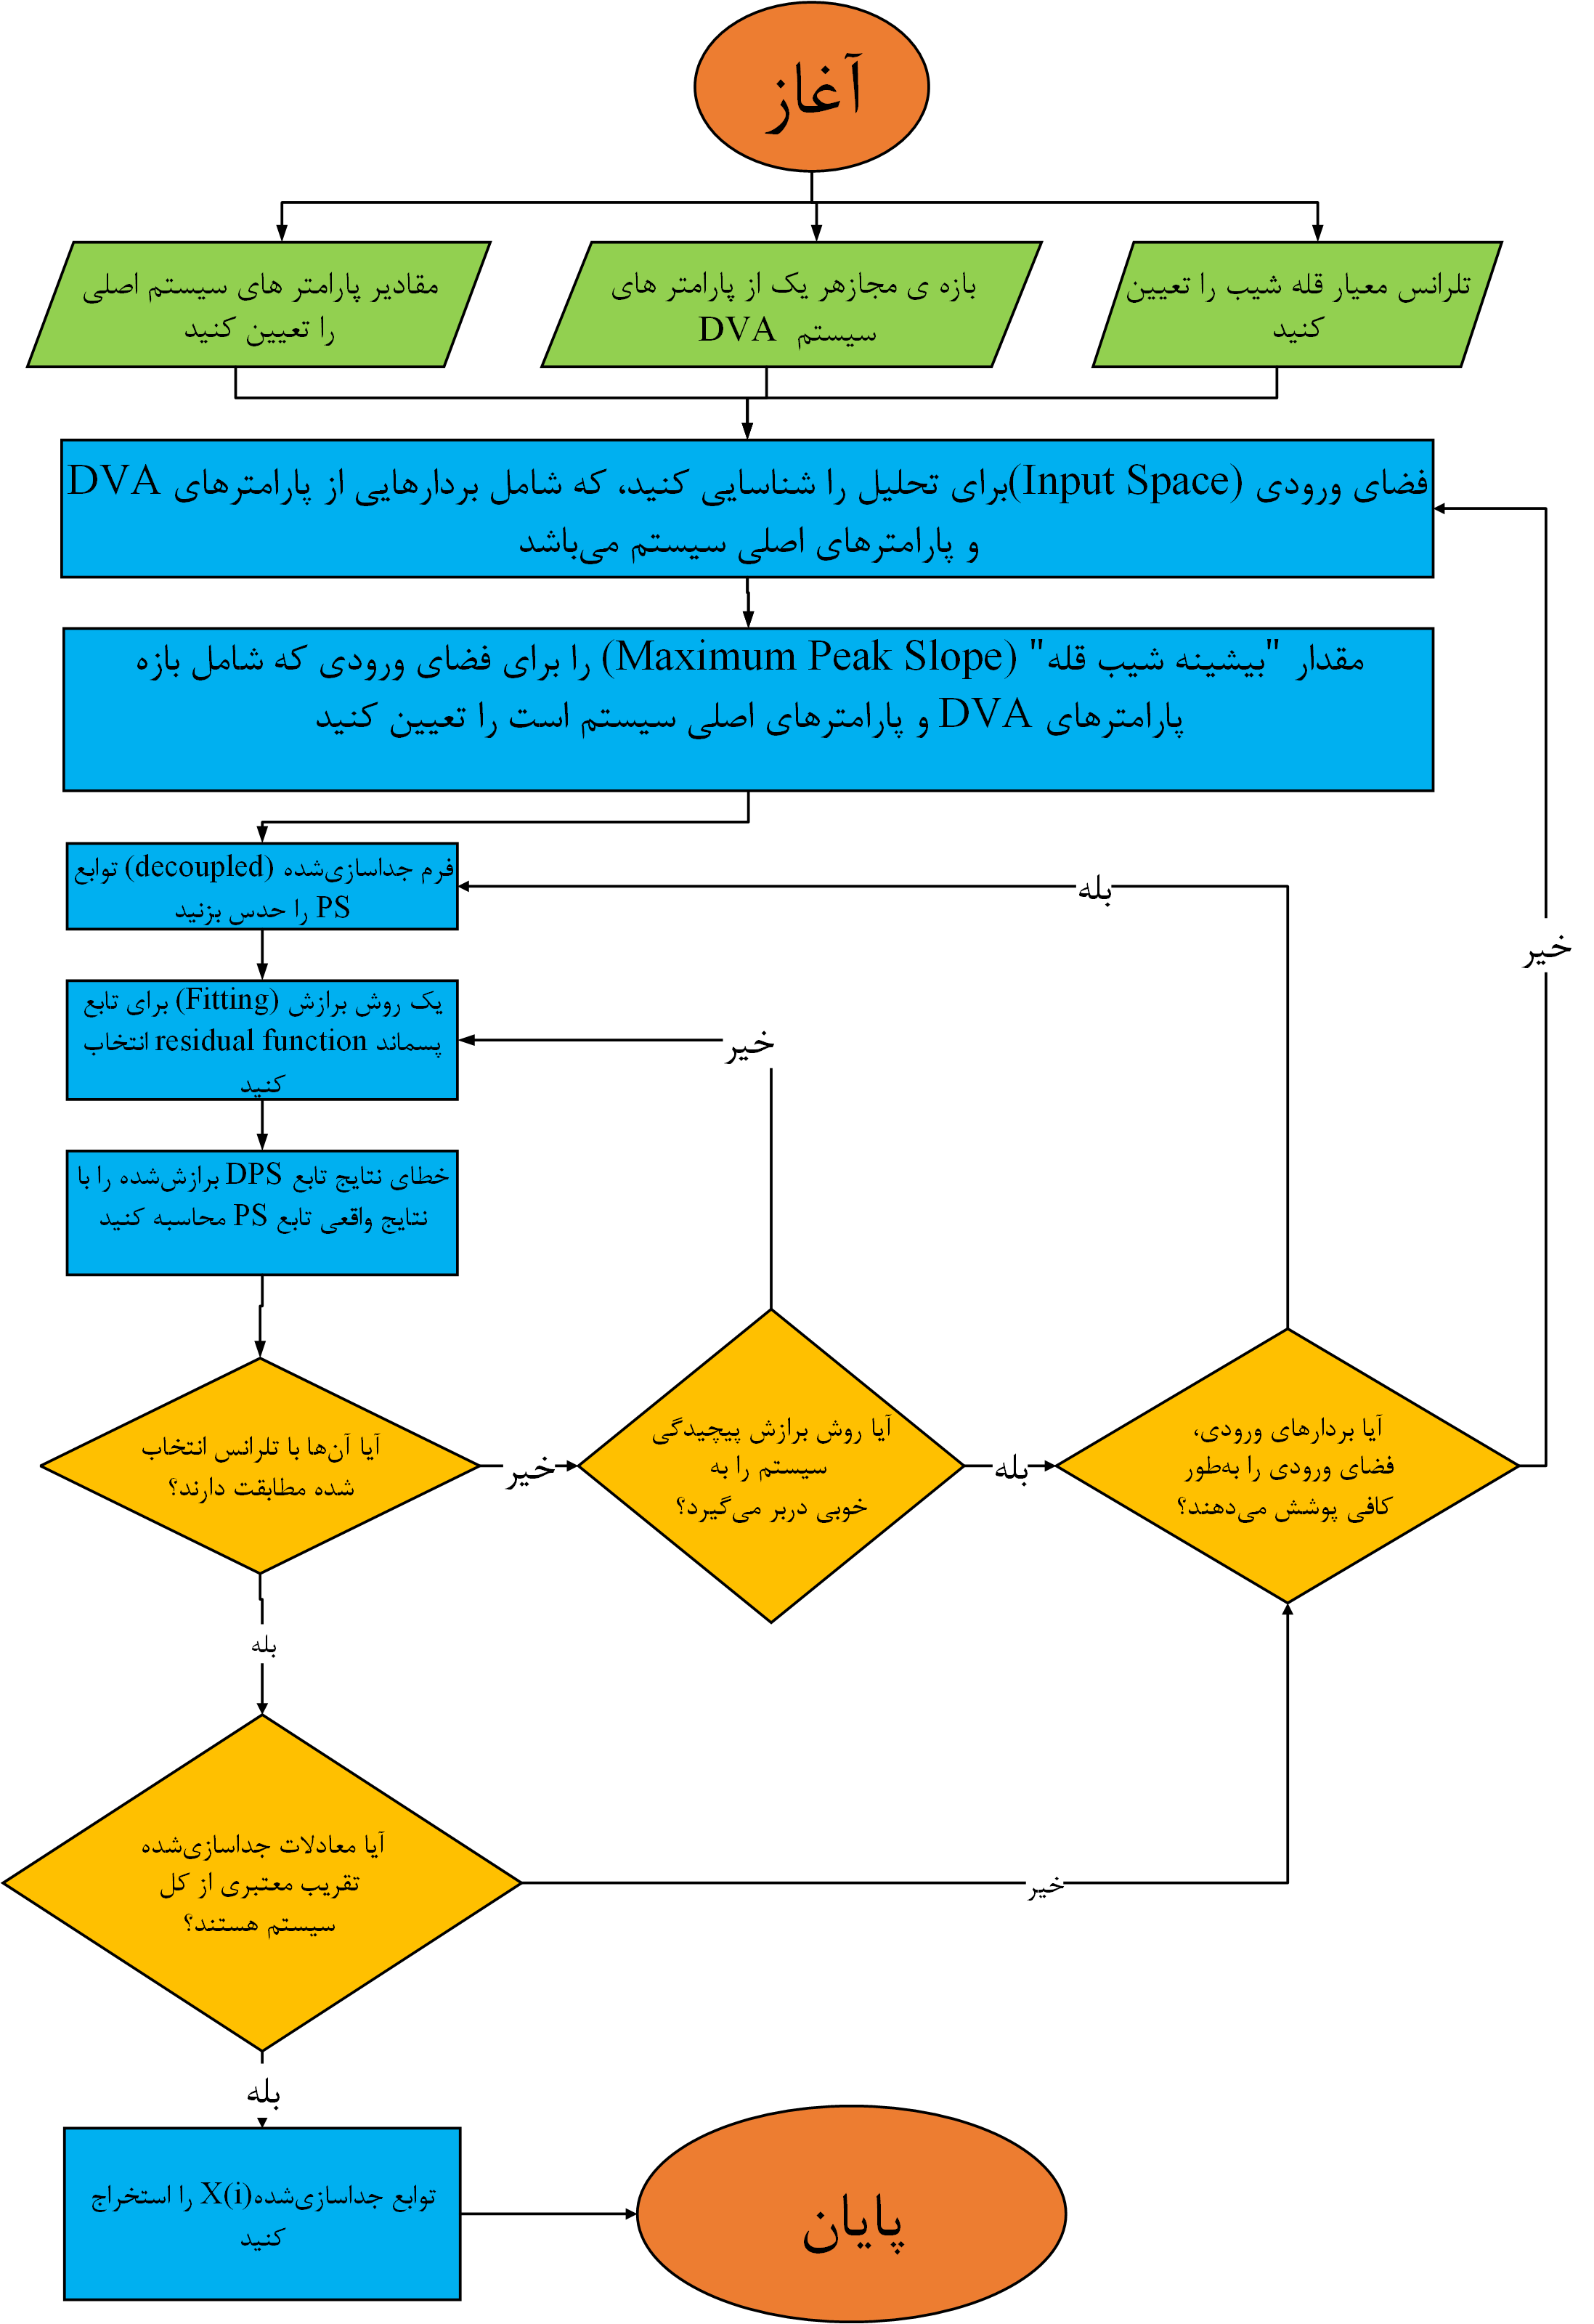
\includegraphics[width=\textwidth]{picture1.png}
        \caption{فلوچارت الگوریتم استخراج توابع جداسازی‌شده $\mathrm{DPS}^{(k)}$ از سیستم دینامیکی کاملاً کوپل شده.}
        \label{fig:dps-subfig1}
    \end{subfigure}
\end{figure}

\begin{figure}[H]
    \centering
    \begin{subfigure}[b]{\textwidth}
        \centering
        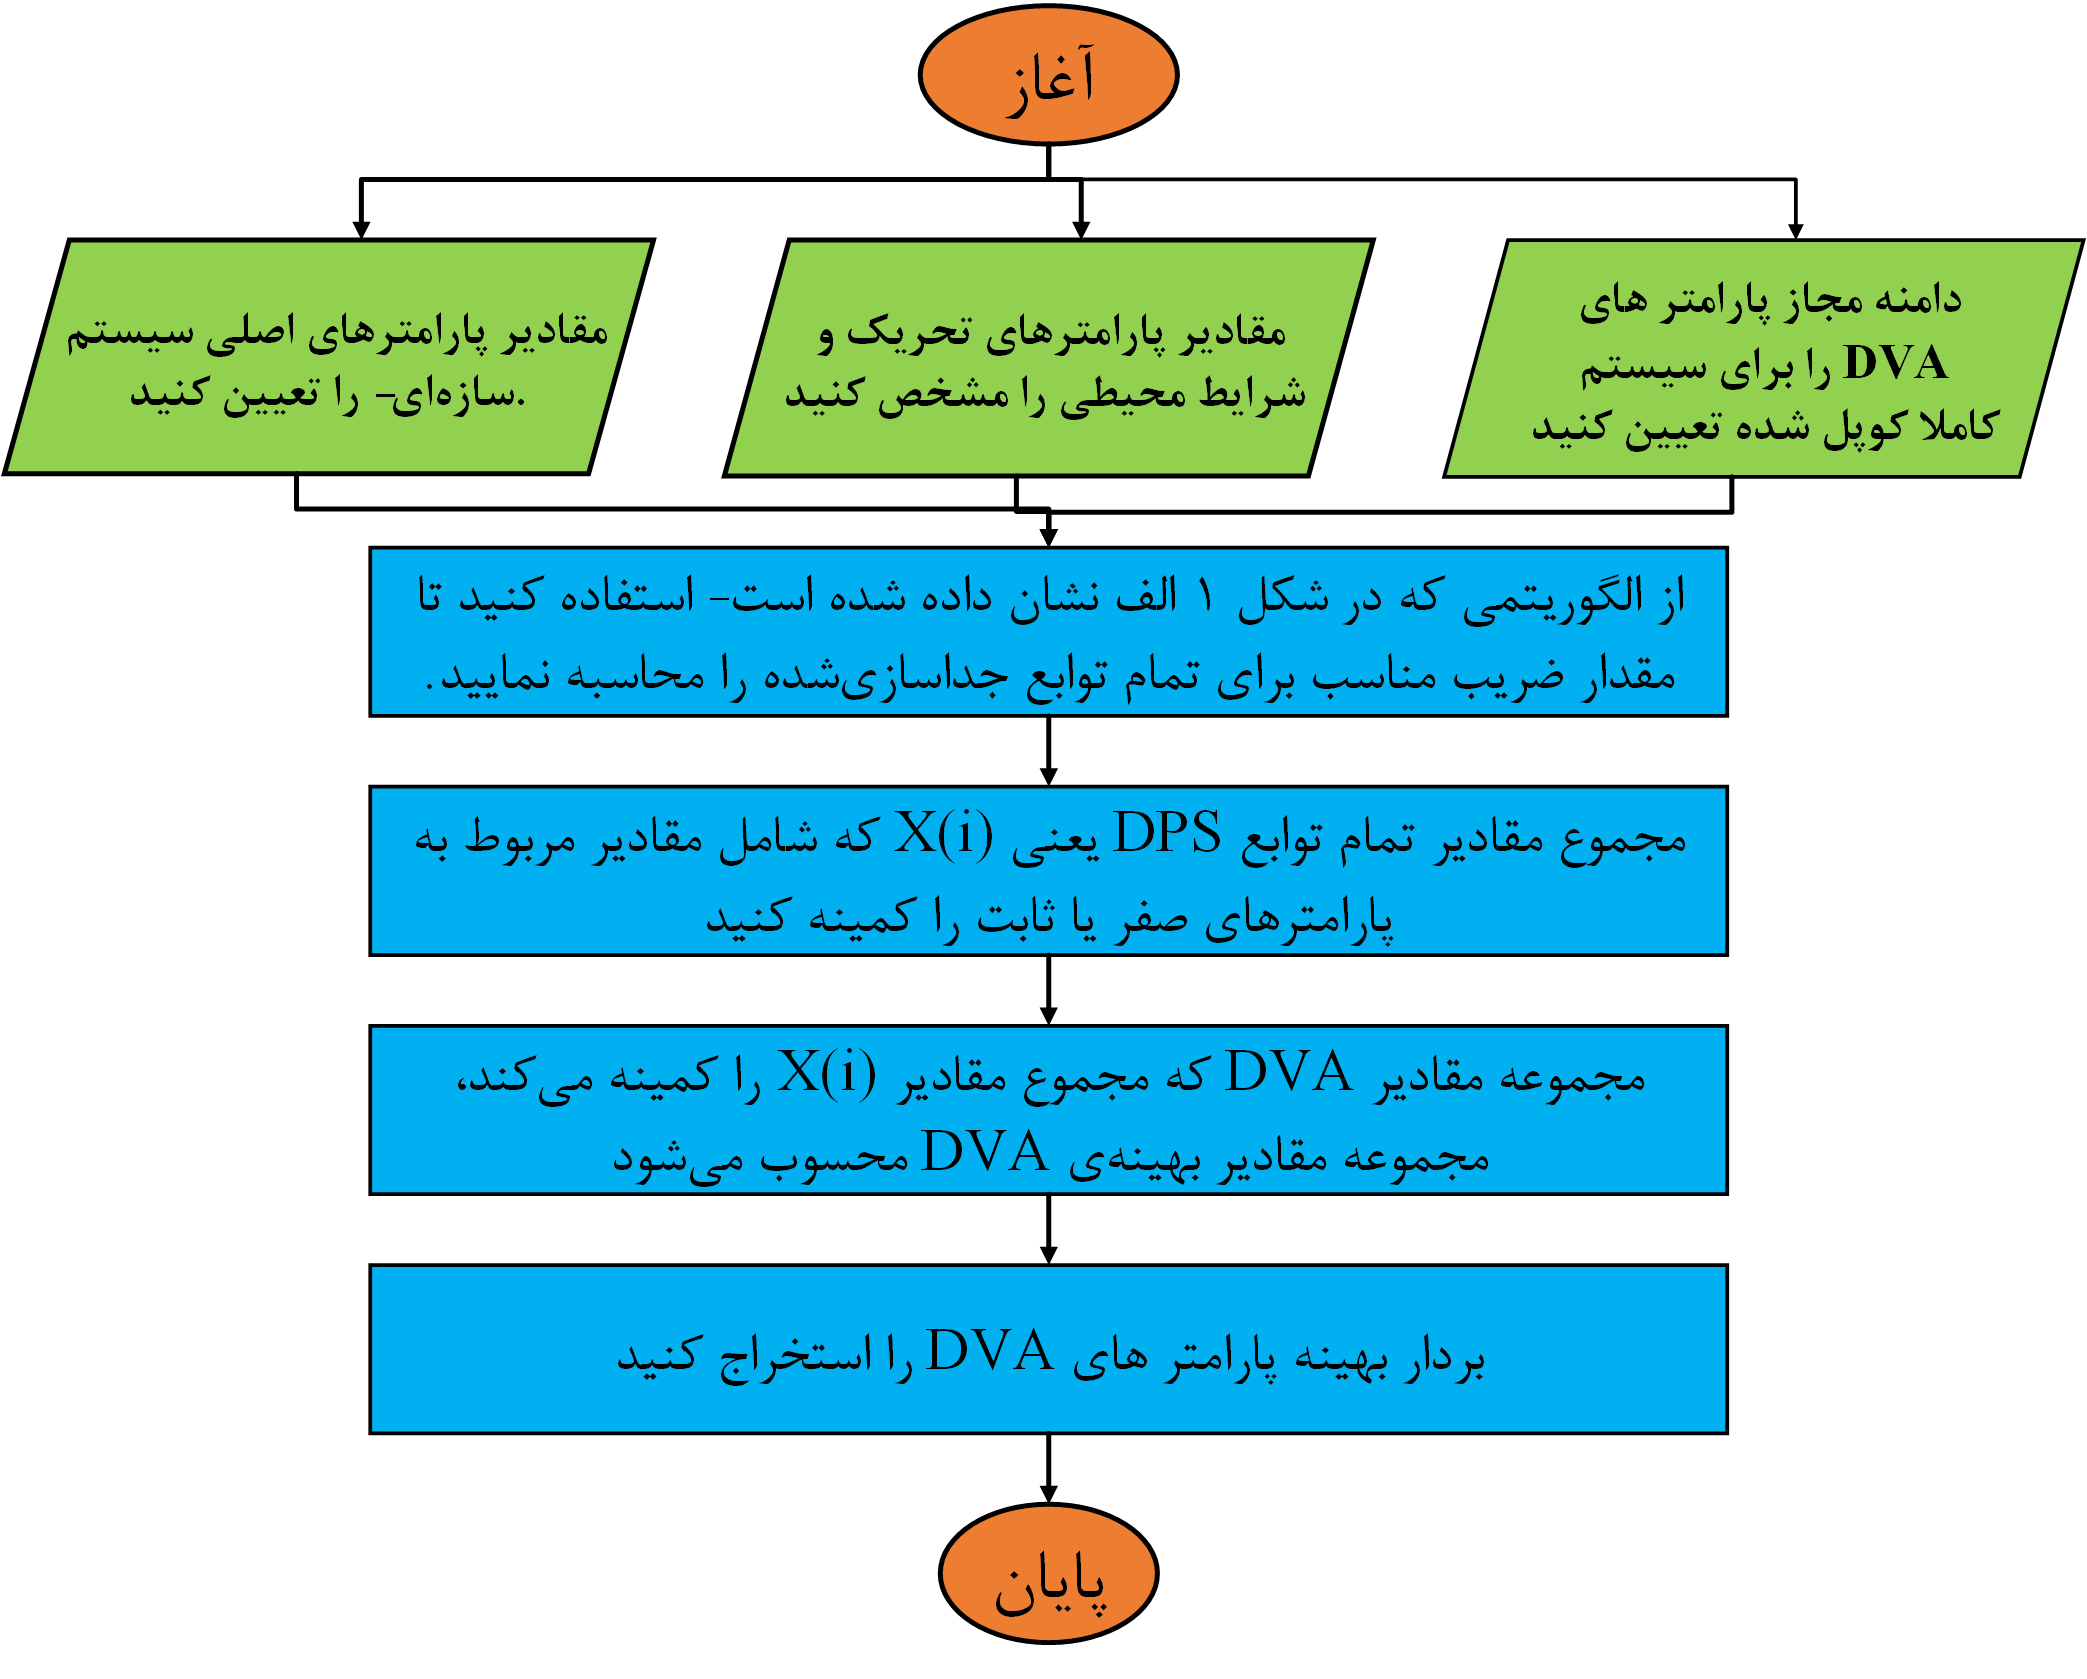
\includegraphics[width=\textwidth]{picture2.png}
        \caption{روند تعیین پارامترهای بهینه \lr{DVA} با استفاده از توابع جانشین جداسازی‌شده.}
        \label{fig:dps-subfig2}
    \end{subfigure}
    \caption{نمای کلی از الگوریتم پیشنهادی شامل (الف) استخراج توابع جداسازی‌شده \lr{DPS} از مدل کامللا کوپل شده و (ب) بهینه‌سازی پارامترهای جاذب بر پایه این توابع. هر زیرشکل در صورت نیاز به‌صورت مجزا در یک صفحه نمایش داده می‌شود.}
    \label{fig:DPS-algorithm}
\end{figure}
% --- پایان بخش ---

\section{تحلیل نمونه‌ای از سیستم کاملاً کوپله‌شده \lr{1DOF–1DOF}}

\subsection{مرور کلی و پیکربندی سیستم}

برای ارزیابی چارچوب پیشنهادی بهینه‌سازی مبتنی بر مدل جانشین و معیار \lr{Peak-Slope (PS)}، یک سیستم مکانیکی کاملاً کوپله‌شده با یک درجه آزادی برای سازه اصلی و یک درجه آزادی برای جاذب انتخاب شده است. این سیستم به‌عنوان یک نمونه‌ی مرجع طراحی شده تا تمامی عناصر پایه‌ای موجود در سازه‌های ارتعاشی را در خود جای دهد؛ از جمله جرم‌های اولیه و ثانویه، فنرها، میراگرها و المان‌های \lr{Inerter}.

اصطلاح "کاملاً کوپله‌شده" در اینجا بدین معناست که نه‌تنها سیستم اصلی و جاذب دینامیکی به‌صورت مستقیم به یکدیگر متصل‌اند، بلکه هر دو به‌طور هم‌زمان به گره‌های پایه‌ای ساختار نیز کوپله شده‌اند. این اتصال دوجانبه، امکان تبادل کامل نیرو و انرژی بین اجزای مختلف را فراهم می‌سازد و رفتار دینامیکی جامع‌تری نسبت به مدل‌های ساده‌شده ارائه می‌دهد.

چنین پیکربندی‌ای نماینده‌ای مناسب از بسیاری کاربردهای واقعی در مهندسی مکانیک و سازه است و می‌تواند به‌عنوان سکوی آزمون ایده‌آلی برای بررسی کارایی الگوریتم پیشنهادی به‌کار رود. به‌ویژه، حضور هم‌زمان المان \lr{Inerter} در کنار فنر و میراگر، پیچیدگی مدل را افزایش داده و آن را به شرایط واقعی نزدیک‌تر می‌سازد.

به‌منظور درک بهتر ساختار سیستم، نمودار شماتیک آن در شکل \lr{Fig.~\ref{fig:fully-coupled-1dof}} ارائه شده است که چیدمان اجزا و نحوه اتصال آن‌ها را به‌صورت تصویری نمایش می‌دهد.

\begin{figure}[H]
\centering
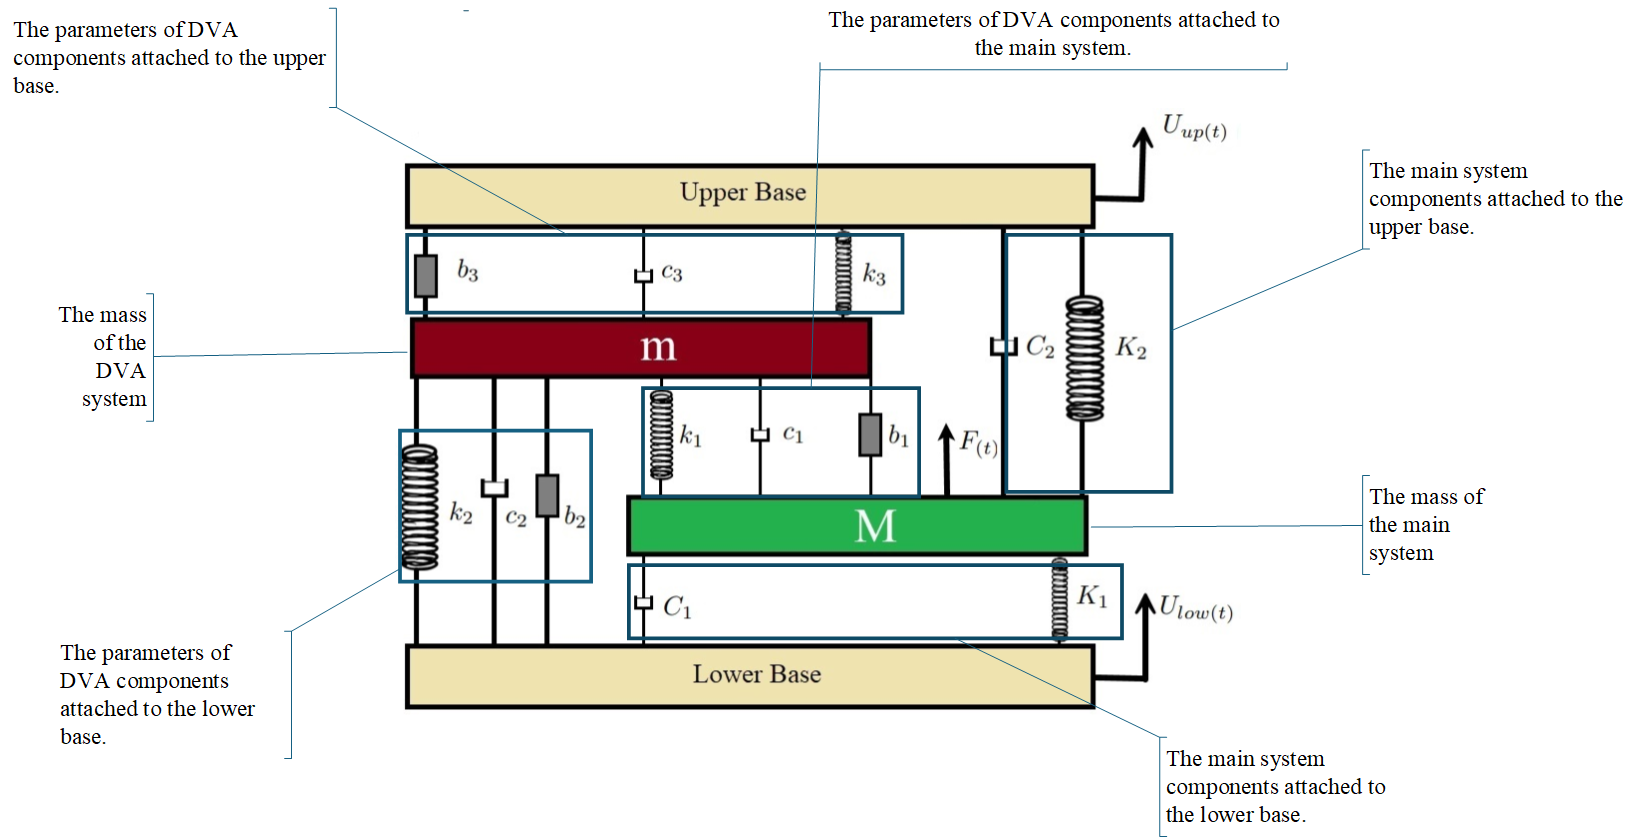
\includegraphics[width=1.1\textwidth]{picture3.png}
\caption{نمای شماتیک از یک سیستم کاملاً کوپله‌شده \lr{1DOF–1DOF}}
\label{fig:fully-coupled-1dof}
\end{figure}



% --- پایان بخش ---

\subsection{مدل‌سازی ریاضی سیستم همراه با مفروضات}

برای تحلیل دقیق و در عین حال ساده‌سازی‌شده، سیستم اصلی به‌صورت یک سازه با یک درجه آزادی (\lr{1DOF}) مدل‌سازی شده است که شامل جرم، فنر و میراگر می‌باشد و این اجزا به پایه‌های بالایی و پایینی متصل شده‌اند. مفروضات اصلی این مدل‌سازی به شرح زیر است:

\begin{enumerate}
  \item رفتار الاستیک خطی برای فنرها با سختی‌های \lr{$K_1$} و \lr{$K_2$}.
  \item میرایی ساختاری خطی برای میراگرها با ضرایب \lr{$C_1$} و \lr{$C_2$}.
  \item حرکت سیستم به‌صورت صرفاً انتقالی در نظر گرفته شده و اثرات چرخشی نادیده گرفته شده‌اند.
\end{enumerate}

این مفروضات به‌منظور دستیابی به مدلی قابل تحلیل و بهینه‌سازی در زمینه کنترل ارتعاش به کار گرفته شده‌اند. پایه‌های بالایی و پایینی، بسته به پیچیدگی سیستم، می‌توانند به‌صورت پایه‌های ثابت یا به‌صورت جرم‌های اضافی مدل شوند. جاذب دینامیکی ارتعاش (\lr{DVA}) نیز به‌صورت یک سیستم \lr{1DOF} شامل جرم، فنر، میراگر و المان \lr{Inerter} مدل‌سازی شده و به‌طور کامل با سیستم اصلی و پایه‌ها کوپله شده است. مفروضات مدل‌سازی برای جاذب مشابه با ساختار اصلی در نظر گرفته شده‌اند.

متغیر کلی سیستم با نماد $q$ تعریف می‌شود و جابه‌جایی‌های سیستم اصلی و جاذب دینامیکی در زمان $t$ به‌ترتیب با $U(t)$ و $u(t)$ نمایش داده می‌شوند. بنابراین بردار جابه‌جایی، سرعت و شتاب به‌صورت زیر تعریف می‌گردند:

\begin{equation}
q = 
\begin{bmatrix}
U(t) \\
u(t)
\end{bmatrix}, \quad
\dot{q} = 
\begin{bmatrix}
\dot{U}(t) \\
\dot{u}(t)
\end{bmatrix}, \quad
\ddot{q} = 
\begin{bmatrix}
\ddot{U}(t) \\
\ddot{u}(t)
\end{bmatrix}
\end{equation}

معادله حرکت سیستم را می‌توان به‌صورت ابعادی و مطابق رابطه زیر بیان کرد:

\begin{equation}
\left[M\right]\ddot{q} + 2\zeta_{dc}\omega_{dc}\left[C\right]\dot{q} + \omega_{dc}^2\left[K\right]q = \left[F\right]
\end{equation}

در این معادله، ماتریس‌های جرم، میرایی و سختی به‌صورت زیر تعریف می‌شوند:

\begin{equation}
\left[M\right] = 
\begin{bmatrix}
1 + \beta_1 & -\beta_1 \\
-\beta_1 & \mu + \beta_1 + \beta_2 + \beta_3
\end{bmatrix}
\end{equation}

\begin{equation}
\left[C\right] = 
\begin{bmatrix}
1 + N + \nu_1 & -\nu_1 \\
-\nu_1 & \nu_1 + \nu_2 + \nu_3
\end{bmatrix}
\end{equation}

\begin{equation}
\left[K\right] = 
\begin{bmatrix}
1 + \Lambda + \lambda_1 & -\lambda_1 \\
-\lambda_1 & \lambda_1 + \lambda_2 + \lambda_3
\end{bmatrix}
\end{equation}

بردار نیروهای ورودی به سیستم نیز به‌صورت زیر تعریف می‌گردد:

\begin{align}
\left[F\right] = 
\begin{bmatrix}
F^\prime + 2\zeta_{dc}\omega_{dc} \left( \dot{U}_{Low} + N \dot{U}_{Up} \right) + \omega_{dc}^2 \left( U_{Low}(t) + \Lambda U_{Up}(t) \right) \\
\beta_2 \ddot{U}_{Low} + \beta_3 \ddot{U}_{Up} + 2\zeta_{dc}\omega_{dc} \left( \nu_2 \dot{U}_{Low} + \nu_3 \dot{U}_{Up} \right) + \omega_{dc}^2 \left( \lambda_2 U_{Low}(t) + \lambda_3 U_{Up}(t) \right)
\end{bmatrix}
\end{align}

این مدل‌سازی، با وجود سادگی نسبی، قابلیت کافی برای بررسی پدیده‌های دینامیکی پیچیده از جمله اثر \lr{Inerter}، میرایی ساختاری، و تعامل کامل بین جاذب و سیستم اصلی را فراهم می‌سازد. چارچوب ارائه‌شده پایه تحلیل‌های بعدی در زمینه معیار \lr{Peak-Slope} و روش بهینه‌سازی مبتنی بر مدل جانشین را شکل خواهد داد.

% --- پایان بخش ---

\subsection{تعریف پارامترهای بدون‌بُعد سیستم}

به‌منظور تحلیل نرمال‌سازی‌شده و بهینه‌سازی مؤثر، پارامترهای ابعادی سیستم به‌دقت تعریف شده‌اند. این نرمال‌سازی باعث کاهش تعداد متغیرهای مستقل و افزایش قابلیت تعمیم نتایج به انواع مختلفی از سازه‌ها می‌شود.

\subsubsection*{نسبت جرم}

نسبت جرم با نماد $\mu$ تعریف می‌شود به‌صورت زیر:

\begin{equation}
\mu \equiv \frac{m}{M}
\end{equation}

که در آن، $m$ جرم جاذب یا \lr{Inerter} و $M$ جرم اصلی سیستم است.

\subsubsection*{نسبت‌های \lr{Inerter}}

برای ضرایب \lr{Inerter}، سه نسبت $\beta_1$، $\beta_2$ و $\beta_3$ به‌صورت زیر تعریف می‌شوند:

\begin{equation}
\beta_i \equiv \frac{b_i}{M}, \quad i=1,2,3
\end{equation}

که $b_i$ ضرایب \lr{Inerter} و $M$ جرم اصلی است.

\subsubsection*{نسبت‌های سختی}

نسبت‌های سختی شامل $\lambda_1$، $\lambda_2$، $\lambda_3$ و $\Lambda$ هستند که به‌صورت زیر تعریف می‌شوند:

\begin{equation}
\lambda_i \equiv \frac{k_i}{K_1}, \quad i=1,2,3 \qquad \Lambda \equiv \frac{K_2}{K_1}
\end{equation}

که در آن $k_i$ ضرایب سختی مربوط به جاذب و $K_1$ و $K_2$ ضرایب سختی در سیستم پایه هستند.

\subsubsection*{نسبت‌های میرایی}

به‌طور مشابه، نسبت‌های میرایی با نمادهای $\nu_1$، $\nu_2$، $\nu_3$ و $N$ تعریف می‌شوند:

\begin{equation}
\nu_i \equiv \frac{c_i}{C_1}, \quad i=1,2,3 \qquad N \equiv \frac{C_2}{C_1}
\end{equation}

که در آن $c_i$ ضرایب میرایی اجزای جاذب و $C_1$ و $C_2$ ضرایب میرایی سیستم اصلی هستند.

\subsubsection*{فرکانس طبیعی و نسبت میرایی نرمال‌شده}

فرکانس طبیعی نرمال‌شده سیستم پایه ($\omega_{dc}$) و نسبت میرایی نرمال‌شده ($\zeta_{dc}$) به‌صورت زیر تعریف می‌شوند:

\begin{equation}
\omega_{dc} \equiv \sqrt{\frac{K_1}{M}}, \qquad \zeta_{dc} \equiv \frac{C_1}{2M\omega_{dc}}
\end{equation}

این دو کمیت به‌عنوان مقیاس‌های پایه برای نرمال‌سازی پاسخ فرکانسی و پارامترهای سیستم به کار می‌روند.

\subsubsection*{نیروی نرمال‌شده}

برای نرمال‌سازی نیروی خارجی اعمال‌شده، از عبارت زیر استفاده می‌شود:

\begin{equation}
F_t' \equiv \frac{F_t}{M}
\end{equation}

که در آن $F_t$ نیروی اعمال‌شده به سیستم و $M$ جرم اصلی است.

\subsubsection*{فرکانس تحریک نرمال‌شده}

در نهایت، فرکانس تحریک نرمال‌شده $\Omega$ به‌صورت نسبت بین فرکانس تحریک $\omega$ و فرکانس طبیعی نرمال‌شده سیستم پایه تعریف می‌شود:

\begin{equation}
\Omega \equiv \frac{\omega}{\omega_{dc}}
\end{equation}

استفاده از این پارامترها در مراحل بعدی به‌ویژه در ساخت مدل‌های جانشین، تحلیل حساسیت و انجام بهینه‌سازی، موجب تسهیل محاسبات و افزایش دقت مدل‌سازی می‌گردد.

% --- پایان بخش ---

\subsection{راه‌حل‌های نیمه‌تحلیلی برای تحریک هارمونیک و حرکت هم‌زمان}

در این بخش، از روشی نیمه‌تحلیلی برای به‌دست‌آوردن پاسخ سیستم استفاده می‌شود. در این رویکرد، ابتدا ساختاری کلی برای پاسخ متغیرهای تعمیم‌یافته در نظر گرفته می‌شود که فرم آن معلوم ولی ضرایب آن نامعلوم هستند. سپس با اعمال شرایط مرزی و اولیه، ضرایب ناشناخته مشخص می‌گردند. تحلیل بر این فرض استوار است که تحریک هارمونیک و حرکت پایه‌ها هم‌زمان و هماهنگ هستند، به‌عبارتی همه مؤلفه‌ها با فرکانس یکسان $\omega$ و در فاز زمانی یکسان عمل می‌کنند.

پاسخ حالت پایدار متغیر تعمیم‌یافته سیستم به صورت زیر نوشته می‌شود:

\begin{equation}
q = 
\begin{bmatrix}
U(t) \\
u(t)
\end{bmatrix}
=
\begin{bmatrix}
A \\
a
\end{bmatrix}
e^{j\omega t}
\end{equation}

که در آن $\omega$ فرکانس تحریک، و $A$ و $a$ به‌ترتیب دامنه ارتعاش در سیستم اصلی و جاذب دینامیکی ارتعاش (\lr{DVA}) هستند.

تحریک هارمونیک جرم سیستم اصلی و حرکت هارمونیک پایه‌ها نیز به‌صورت زیر تعریف می‌شود:

\begin{equation}
F'(t) = f\, e^{j\omega t}
\end{equation}

\begin{equation}
U_{\mathrm{Low}}(t) = A_{\mathrm{Low}}\, e^{j\omega t}
\end{equation}

\begin{equation}
U_{\mathrm{Up}}(t) = A_{\mathrm{Up}}\, e^{j\omega t}
\end{equation}

در این روابط، $f$ دامنه نیروی تحریک‌کننده است، در حالی که $A_{\mathrm{Low}}$ و $A_{\mathrm{Up}}$ به‌ترتیب دامنه‌های حرکت پایه‌های پایین و بالا را نشان می‌دهند.

با جایگذاری این مقادیر در معادله حرکت سیستم، فرم کلی پاسخ به‌صورت زیر بازنویسی می‌شود:

\begin{equation}
\begin{bmatrix}
A \\
a
\end{bmatrix}
=
\omega_{dc}^2 \left(
\left(
-\Omega^2 [M]
+ 2j\omega \zeta_{dc} \Omega [C]
+ [K]
\right) e^{j\omega t}
\right)^{-1}
\left[f\right]
\end{equation}

که در آن:
\begin{enumerate}
  \item $[M]$ ماتریس جرم،
  \item $[C]$ ماتریس میرایی،
  \item $[K]$ ماتریس سختی،
  \item $\zeta_{dc}$ میرایی معادل،
  \item $\omega_{dc}$ فرکانس مشخصه دینامیکی سیستم،
  \item $\Omega$ نسبت فرکانس تحریک به فرکانس طبیعی سیستم است.
\end{enumerate}

این بیان نیمه‌تحلیلی امکان استخراج دقیق پاسخ دامنه‌ای سیستم را در حضور تحریک هارمونیک فراهم می‌سازد و مبنای تحلیل عملکرد جاذب در فضای فرکانس را تشکیل می‌دهد.

% --- پایان بخش ---

\subsection{پارامترهای سیستم}

به‌منظور ارزیابی چارچوب پیشنهادی، یک تحلیل عددی با استفاده از پارامترهایی دلخواه برای سیستم اصلی انجام شده است. این پارامترها در جدول \ref{tab:main-system-parameters} ارائه شده‌اند.

\begin{table}[H]
\centering
\caption{ مقادیر عددی سیستم مورد مطالعه}
\label{tab:main-system-parameters}
\begin{tabular}{cc}
\hline
سیستم اصلی & مقدار \\
\hline
$\Lambda$ & $1$ \\
$N$ & $1$ \\
$A_{Up} = A_{Low}$ & $0.0001$ \\
$F$ & $100$ \\
$\omega_{dc}$ & $1000$ \\
$\zeta_{dc}$ & $0.01$ \\
\hline
\end{tabular}
\end{table}

مقادیر فوق به‌عنوان پایه‌ای برای آزمون عملکرد الگوریتم \lr{DPS} در شرایط کنترل‌شده استفاده شده‌اند. در ادامه، تحلیل‌های عددی و نتایج حاصل از اعمال روش پیشنهادی بر این سیستم بررسی خواهند شد.

% --- پایان بخش ---

\subsection{تابع جداسازی‌شده شیب-قله (\lr{Decoupled Peak-Slope})}

رفتار دینامیکی سیستم در چارچوب پیشنهادی با استفاده از تابع \lr{DPS} مدل‌سازی می‌شود؛ تابعی که نقش مرکزی در بهینه‌سازی دارد و به‌صورت مجموعی از ده زیرتابع مستقل تعریف می‌گردد. هر زیرتابع نمایانگر سهم یک پارامتر مشخص از سیستم در معیار کلی \lr{Peak-Slope} است:

\begin{equation}
\mathrm{DPS} = \sum_{i=1}^{10} X_i(p_i)
\end{equation}

در این رابطه، هر $X_i(p_i)$ تابعی از پارامتر خاص $p_i$ بوده و پارامترهایی نظیر $\mu$، $\beta_1$، $\lambda_1$، $\nu_1$، $\beta_2$، $\lambda_2$، $\nu_2$، $\beta_3$، $\lambda_3$ و $\nu_3$ را پوشش می‌دهد. پارامترهای اصلی سیستم (ساختار و تحریک)، به‌عنوان بخش‌های ثابت مدل واقعی، از تحلیل خارج شده‌اند تا تمرکز صرفاً بر متغیرهای قابل تنظیم جاذب باشد.

\subsubsection{شرایط اولیه}

برای شروع فرآیند تکرار، مقدار اولیه هر زیرتابع به‌صورت یکسان تعیین می‌شود:

\begin{equation}
X_i^{(0)} = X_{i,0},\quad \forall i = 1,\ldots,10
\end{equation}

که در آن $X_{i,0}$ مقدار اولیه زیرتابع $X_i$ در گام $k=0$ است.

\subsubsection{محدوده تعریف پارامترها}

هر پارامتر $p_j$ در بازه مشخصی تعریف می‌شود که به‌صورت گسسته و با گام ثابت نمونه‌برداری می‌شود:

\begin{equation}
p_j \in \left\{p_{j,i},\ p_{j,i}+\Delta p_j,\ \ldots,\ p_{j,f}\right\},\quad \forall j = 1,\ldots,10
\end{equation}

در این رابطه، $p_{j,i}$ و $p_{j,f}$ به‌ترتیب مقادیر ابتدایی و انتهایی پارامتر $p_j$ هستند و $\Delta p_j$ اندازه گام تغییرات آن است.

\subsubsection{روند تکراری به‌روزرسانی زیرتوابع}

به‌منظور محاسبه مقدار هر زیرتابع در گام بعدی، از مقدار \lr{DPS} و مجموع سایر زیرتوابع در گام قبلی استفاده می‌شود. رابطه به‌روزرسانی به‌صورت زیر تعریف می‌شود:

\begin{equation}
X_i^{(k+1)}(p_i) = \mathrm{DPS}(p_i,\text{سایر پارامترها}) - \sum_{\substack{j=1 \\ j \ne i}}^{10} X_j^{(k)}(\text{سایر پارامترها})
\end{equation}

با شرایط:
\[
\left\{
\begin{aligned}
& p_i \in \left\{p_{i,i},\ p_{i,i}+\Delta p_i,\ \ldots,\ p_{i,f} \right\} \\
& i = 1,2,\ldots,10 \\
& k = 0,1,2,\ldots
\end{aligned}
\right.
\]

در این ساختار، به‌ازای هر پارامتر متغیر، مقدار تابع مربوطه با تفریق مجموع سایر زیرتوابع از مقدار کلی \lr{DPS} محاسبه می‌شود. این فرآیند به‌صورت تکراری انجام شده و تا رسیدن به همگرایی ادامه می‌یابد.


\subsubsection{مدل‌سازی جانشین زیرتوابع}

در هر گام، مقدار محاسبه‌شده $X_i^{(k)}(p_i)$ به‌عنوان نقطه داده برای ساخت مدل جانشین مربوط به پارامتر $p_i$ در نظر گرفته می‌شود. برای تقریب رفتار این توابع در طول تکرار، از مدل‌های چندجمله‌ای (مانند رگرسیون چهارم‌درجه) استفاده می‌شود که تعادل مناسبی بین دقت و سرعت محاسباتی فراهم می‌آورند.

این مدل‌های جانشین، پایه اصلی بهینه‌سازی تابع \lr{DPS} را تشکیل می‌دهند و امکان تحلیل سریع، کاهش نیاز به شبیه‌سازی‌های پیچیده، و استخراج پارامترهای بهینه با دقت بالا را فراهم می‌سازند.

% --- پایان بخش ---

\subsection{کارایی برازش چندجمله‌ای}

برای تعیین دقیق‌ترین روش تقریب تابع جزئی \lr{DPS}، عملکرد چندین مدل برازش چندجمله‌ای ارزیابی شد. نتایج این تحلیل در شکل \ref{fig:polyfit-comparison} و جدول \ref{tab:polyfit-error} ارائه شده‌اند. ارزیابی‌ها بر پایه خطای میانگین، انحراف معیار و ریشه میانگین مربعات خطا (\lr{RMSE}) صورت گرفت. در هر زیرنمودار از شکل \ref{fig:polyfit-comparison}، محور افقی بیانگر مقادیر واقعی \lr{PS} و محور عمودی بیانگر مقادیر پیش‌بینی‌شده توسط مدل است. هر نقطه نشان‌دهنده یک مجموعه پارامتر منحصر به‌فرد برای \lr{DVA} است. خط‌چین قرمز، خط برازش کامل یا ایده‌آل را نمایش می‌دهد.

با افزایش درجه چندجمله‌ای، دقت تقریب به‌طور قابل‌ملاحظه‌ای افزایش یافت. برازش خطی (شکل \ref{fig:polyfit-comparison}–الف) بیشترین خطا را نشان داد و مقدار \lr{RMSE} برابر با $1.4430\times10^{-10}$ بود. برازش درجه دوم (شکل \ref{fig:polyfit-comparison}–ب) خطا را به $8.3068\times10^{-11}$ کاهش داد. در ادامه، مدل مکعبی (شکل \ref{fig:polyfit-comparison}–ج) عملکرد بهتری ارائه داد ($\mathrm{RMSE}=1.9874\times10^{-11}$). در نهایت، برازش درجه چهارم (شکل \ref{fig:polyfit-comparison}–د) کمترین میزان خطا را با $\mathrm{RMSE}=2.9908\times10^{-12}$ به‌دست آورد و بیشترین هم‌خوانی با خط برازش کامل را از خود نشان داد.

بنابراین، براساس نتایج کمی و کیفی، چندجمله‌ای مرتبه چهارم به‌عنوان دقیق‌ترین و بهینه‌ترین روش برای تقریب تابع \lr{DPS} انتخاب شد.

\begin{figure}
    \centering
    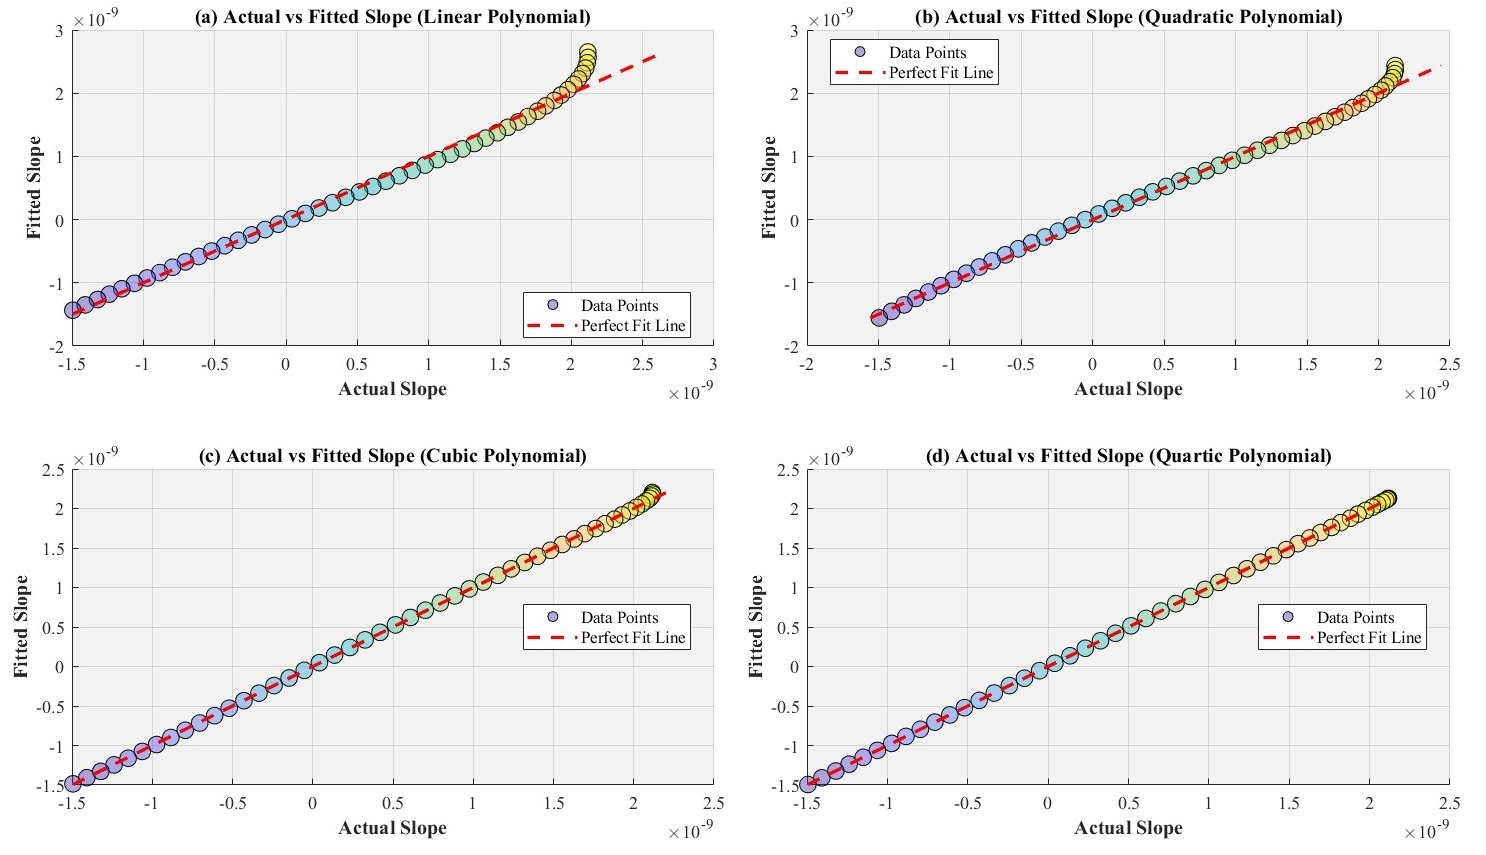
\includegraphics[width=1.1\textwidth]{picture4.png}
    \caption{مقایسه روش‌های برازش چندجمله‌ای برای تابع \lr{DPS}: (الف) خطی، (ب) درجه دوم، (ج) درجه سوم، (د) درجه چهارم. خط‌چین قرمز: برازش ایده‌آل، نقاط: مقادیر واقعی در برابر مقادیر پیش‌بینی‌شده}
    \label{fig:polyfit-comparison}
\end{figure}


\begin{table}[h]
    \centering
    \caption{مقایسه آماری خطای برازش مدل‌های چندجمله‌ای}
    \label{tab:polyfit-error}
    \begin{tabular}{cccc}
        \hline
        \lr{Fitting Method} & \lr{Mean Error} & \lr{STD} & \lr{RMSE} \\
        \hline
        \lr{Linear Polynomial}   & $9.6730\times10^{-11}$ & $1.0819\times10^{-10}$ & $1.4430\times10^{-10}$ \\
        \lr{Quadratic Polynomial} & $5.8807\times10^{-11}$ & $5.9277\times10^{-11}$ & $8.3068\times10^{-11}$ \\
        \lr{Cubic Polynomial}     & $1.2789\times10^{-11}$ & $1.5370\times10^{-11}$ & $1.9874\times10^{-11}$ \\
        \lr{Quartic Polynomial}   & $1.5188\times10^{-12}$ & $2.6031\times10^{-12}$ & $2.9908\times10^{-12}$ \\
        \hline
    \end{tabular}
\end{table}

% --- پایان بخش ---

\section{تحلیل مرجع \lr{DPS} در یک سیستم کاملاً کوپله \lr{1DOF–1DOF}}

برای ارزیابی عملکرد چارچوب پیشنهادی \lr{DPS}، یک الگوریتم ژنتیک (\lr{Genetic Algorithm} یا \lr{GA}) با شرایط طراحی یکسان پیکربندی شد تا به‌عنوان مبنای مقایسه عمل کند. پارامترهای الگوریتم \lr{GA} شامل اندازه جمعیت برابر با ۱۵۰، تعداد نسل‌ها ۲۰، احتمال تلاقی ۰.۷۰ و احتمال جهش ۰.۲۰ در نظر گرفته شدند. تمام پارامترهای جاذب ارتعاش در بازه $[0, 1]$ مقید شدند، به‌جز نسبت جرم $\mu^1$ که در بازه $[0, 0.75]$ محدود شد. هر ارزیابی توسط الگوریتم \lr{GA} نیازمند محاسبه کامل پاسخ فرکانسی سیستم بود، در حالی که روش \lr{DPS} از ارزیابی‌های تحلیلی مبتنی بر مدل جانشین استفاده می‌کند.

برای بررسی رفتار تصادفی \lr{GA}، صد اجرای مستقل با بذرهای تصادفی متفاوت انجام شد. اگرچه در برخی موارد الگوریتم موفق به یافتن مقدار بهینه برای \lr{PS} شد، اما نوسان زیادی در نتایج مشاهده گردید. بهترین مقدار \lr{PS} حاصل از \lr{GA} برابر با $4.3 \times 10^{-5}$، میانگین برابر با $4.4 \times 10^{-5}$ و بدترین نتیجه برابر با $1.4 \times 10^{-4}$ بود. در مقابل، روش \lr{DPS} به‌صورت قطعی و در تنها یک بار اجرا، مقدار $6.9344 \times 10^{-5}$ را برای \lr{PS} به‌دست آورد.

در جدول \ref{tab:DPS-vs-GA} مقایسه‌ای بین مقادیر پارامترهای بهینه حاصل از روش \lr{DPS} و مقادیر حاصل از بهترین، میانگین و بدترین اجرای الگوریتم ژنتیک ارائه شده است. با وجود آنکه مقدار \lr{PS} به‌دست‌آمده از \lr{DPS} کمی بیشتر از بهترین نتیجه \lr{GA} است، اما این نتیجه با سرعت بالا، بدون تصادف، و تنها در یک مرحله محاسبه حاصل شده است.

\begin{table}[H]
\centering
\caption{مقایسه پارامترهای بهینه و مقادیر \lr{PS} بین روش \lr{DPS} و الگوریتم ژنتیک}
\label{tab:DPS-vs-GA}
\begin{latin}
\begin{tabular}{lcccc}
\hline
\textbf{Parameter} & \textbf{DPS Optimum} & \textbf{Best GA} & \textbf{Mean GA} & \textbf{Worst GA} \\
\hline
PS & $6.9344 \times 10^{-5}$ & $4.3 \times 10^{-5}$ & $4.4 \times 10^{-5}$ & $1.4 \times 10^{-4}$ \\
\hline
$\beta^1$ & 0.79 & 0.006 & 0.104 & 0.63 \\
$\beta^2$ & 0.98 & 0.467 & 0.047 & 0.71 \\
$\beta^3$ & 0.47 & 0.338 & 0.422 & 0.31 \\
$\lambda^1$ & 1.99 & 0.96 & 0.89 & 0.23 \\
$\lambda^2$ & 0.83 & 0.62 & 0.57 & 0.72 \\
$\lambda^3$ & 1.68 & 0.57 & 0.43 & 1.00 \\
$\mu^1$ & 0.17 & 0.49 & 0.05 & 0.40 \\
$\nu^1$ & 1.69 & 0.78 & 0.18 & 1.00 \\
$\nu^2$ & 1.49 & 0.13 & 0.54 & 0.97 \\
$\nu^3$ & 2.35 & 0.32 & 0.18 & 0.57 \\
\hline
\end{tabular}
\end{latin}
\end{table}

نمودار شکل \ref{fig:frf-dps-vs-ga} مقایسه‌ای بصری از توابع پاسخ فرکانسی (\lr{FRF}) به‌دست‌آمده از روش \lr{DPS} و سه نمونه‌نماینده از بین صد اجرای \lr{GA} را نمایش می‌دهد: بهترین، میانگین و بدترین حالت. در نتایج مربوط به حالت‌های بهترین و میانگین \lr{GA}، قله‌های پاسخ با تعادل مناسبی تنظیم شده‌اند و مقادیر \lr{PS} به‌دست‌آمده کمی کمتر از مقدار حاصل از \lr{DPS} هستند که نشان‌دهنده موفقیت در تنظیم جاذب می‌باشد. با این حال، نتیجه مربوط به بدترین حالت \lr{GA} عدم تعادل واضحی در قله‌ها نشان می‌دهد، که بیانگر ضعف این روش در تولید پاسخ‌های پایدار است.

این مقایسه به‌خوبی یکی از محدودیت‌های ذاتی روش‌های مبتنی بر \lr{GA} را آشکار می‌سازد: ذات احتمالی این الگوریتم‌ها منجر به تغییرپذیری در کیفیت نتایج می‌شود و برای دستیابی به پاسخ مناسب، نیاز به تکرارهای متعدد دارند. در مقابل، روش \lr{DPS} به‌صورت قطعی، تنها با یک‌بار اجرا و بدون تصادف، پاسخی با کیفیت بالا تولید می‌کند. اگرچه تنظیم قله‌ها در روش \lr{DPS} همیشه بهتر از بهترین اجرای \lr{GA} نیست، اما پایداری، سرعت بالا، و هزینه محاسباتی ناچیز، آن را به گزینه‌ای برتر برای کاربردهای زمان‌حقیقی یا طراحی سریع تبدیل می‌کند.

\begin{figure}[H]
    \centering
    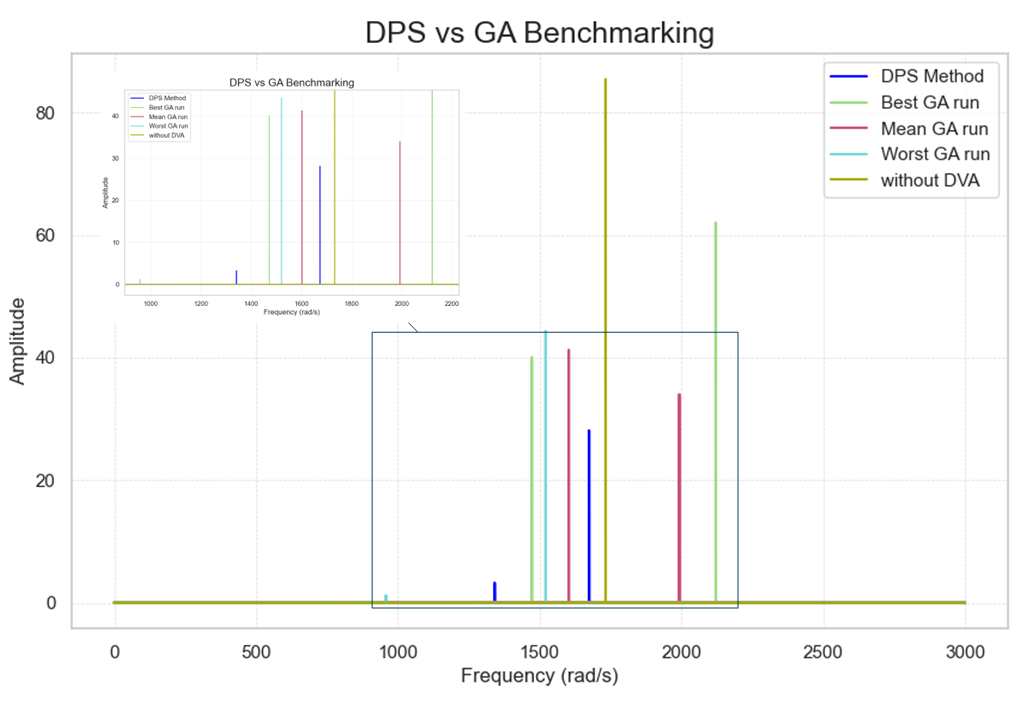
\includegraphics[width=0.85\textwidth]{picture5.png}
    \caption{مقایسه \lr{FRF} بین روش \lr{DPS} و نمونه‌های برتر، میانگین و ضعیف الگوریتم ژنتیک برای سیستم مرجع}
    \label{fig:frf-dps-vs-ga}
\end{figure}

این بررسی نه‌تنها اثربخشی عددی روش پیشنهادی را تأیید می‌کند، بلکه از طریق شواهد بصری و مقایسه‌ای، درک عمیق‌تری از عملکرد آن فراهم می‌آورد؛ به‌ویژه برای خوانندگانی که به دنبال تحلیل‌های کاربردی و قابل تکرار هستند.

% --- پایان بخش ---


\subsection{اعتبارسنجی روش \lr{DPS} در برابر پاسخ‌های تحلیلی سیستم‌های مرتبه پایین}

برای ارزیابی دقت و پایداری روش پیشنهادی \lr{DPS}، یک مطالعه اعتبارسنجی با استفاده از سیستمی با درجه آزادی پایین و دارای راه‌حل تحلیلی شناخته‌شده انجام شد. منطق اصلی این ارزیابی بر پایه این فرض استوار است که اگر فرایند جداسازی پارامترها در چارچوب \lr{DPS} به‌درستی انجام شده باشد، آنگاه معادلات مدل جانشین مشتق‌شده از یک سیستم کاملاً کوپله باید قادر باشند پاسخ‌های صحیحی حتی در مدل‌های ساده‌تر نیز ارائه دهند. چنین نتیجه‌ای نشان‌دهنده جداسازی کامل دینامیک کوپله اولیه خواهد بود.

برای این منظور، از سیستم \lr{1DOF–1DOF} کاملاً کوپله معرفی‌شده در فصل‌های قبل به‌عنوان مبنای ساخت مدل جانشین استفاده شد، اما در مرحله اعتبارسنجی، چارچوب \lr{DPS} بر روی سیستم ساده‌شده‌ای که توسط \lr{Asami et al.} \cite{asami2002analytical} ارائه شده اعمال گردید. در این پیکربندی، جرم اصلی به یک پایه صلب از طریق یک فنر و میرای متصل است و جرم جاذب نیز به جرم اصلی از طریق یک جفت فنر–میرای دیگر متصل می‌گردد (شکل \ref{fig:asami-validation-diagram}).

\begin{figure}[h]
\centering
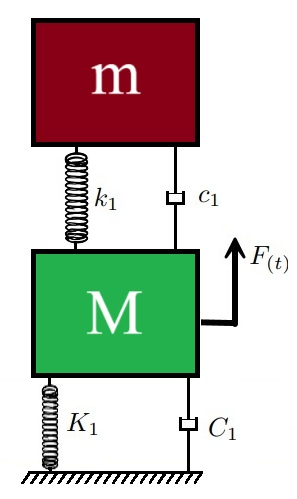
\includegraphics[width=0.25\textwidth]{picture6.png}
\caption{شماتیک سیستم مورد استفاده برای اعتبارسنجی، برگرفته از \lr{Asami et al.} \cite{asami2002analytical}}
\label{fig:asami-validation-diagram}
\end{figure}

در مطالعه‌ی \lr{Asami et al.}، پاسخ‌های تحلیلی مرتبه اول و دوم برای این سیستم استخراج شده‌اند. این پاسخ‌ها به‌عنوان معیارهای مرجع برای مقایسه با نتایج روش \lr{DPS} مورد استفاده قرار گرفتند. در این آزمایش، پارامترهای ساختاری به صورت ثابت در نظر گرفته شدند: فرکانس طبیعی $\Omega_{dc} = 14.14 \Omega$، نسبت میرایی $\zeta_{dc} = 0.24$، نیروی تحریک برابر با ۱۰۰ نیوتن و نسبت جرم $\mu = 0.5$. هدف بهینه‌سازی، تعیین نسبت سختی $\lambda_1$ و نسبت میرایی $\nu_1$ جاذب بود به‌گونه‌ای که معیار \lr{PS} به حداقل برسد. نتایج بهینه‌سازی برای هر سه روش در جدول \ref{tab:asami-comparison} ارائه شده است.

\begin{table}[h]
\centering
\caption{مقایسه پارامترهای بهینه و مقدار \lr{PS} برای سیستم مرجع \lr{Asami et al.} \cite{asami2002optimum}}
\label{tab:asami-comparison}
\begin{tabular}{lccc}
\hline
روش & $\boldsymbol{\lambda}_\mathbf{1}$ & $\boldsymbol{\nu}_\mathbf{1}$ & مقدار \lr{PS} \\
\hline
تحلیلی مرتبه اول (\lr{Asami}) & \lr{0.1525} & \lr{4.568} & \lr{0.59913} \\
تحلیلی مرتبه دوم (\lr{Asami}) & \lr{0.1250} & \lr{4.041} & \lr{0.38587} \\
روش \lr{DPS} پیشنهادی & \lr{0.1280} & \lr{3.381} & \lr{0.04915} \\
\hline
\end{tabular}
\end{table}


شکل \ref{fig:asami-frf-comparison}(الف) تابع پاسخ فرکانسی (\lr{FRF}) حاصل از سه روش را نمایش می‌دهد. همان‌طور که مشاهده می‌شود، هر سه روش پاسخ کلی مشابهی ارائه می‌دهند که صحت چارچوب \lr{DPS} را به‌طور کلی تأیید می‌کند. با این حال، بررسی دقیق‌تر در شکل \ref{fig:asami-frf-comparison}(ب) نشان داده شده که در آن مقادیر معیار \lr{PS} به‌صورت نمودار میله‌ای مقایسه شده‌اند. در این نمودار، مقدار \lr{PS} حاصل از روش \lr{DPS} نزدیک به یک مرتبه کوچکتر از دو روش تحلیلی است که این امر نشان‌دهنده تعادل بهتر بین قله‌ها و تنظیم دقیق‌تر جاذب می‌باشد.

\begin{figure}[h]
\centering
\subfloat[\lr{FRF} حاصل از سه روش مختلف]{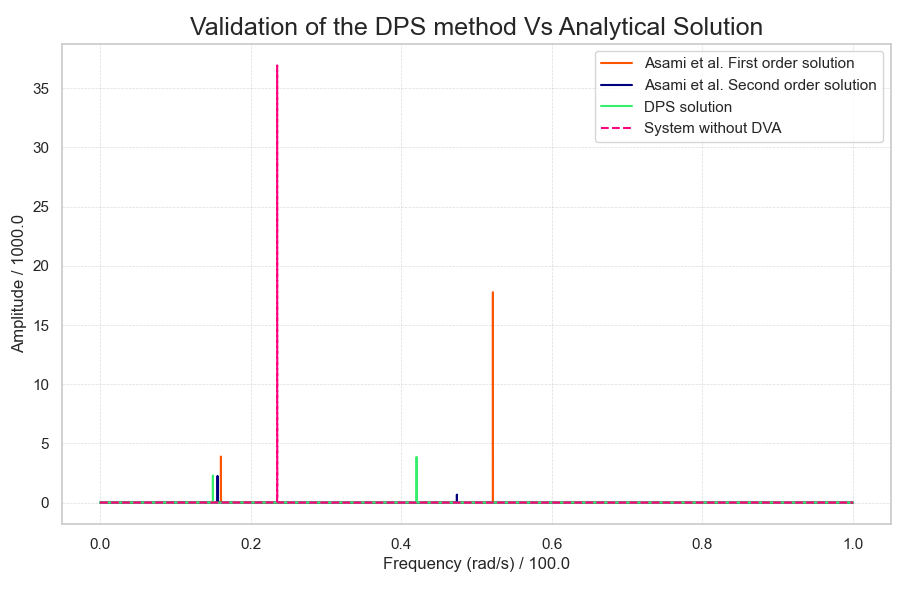
\includegraphics[width=0.5\textwidth]{picture8.png}}
\hfill
\subfloat[مقایسه مقادیر معیار \lr{PS}]{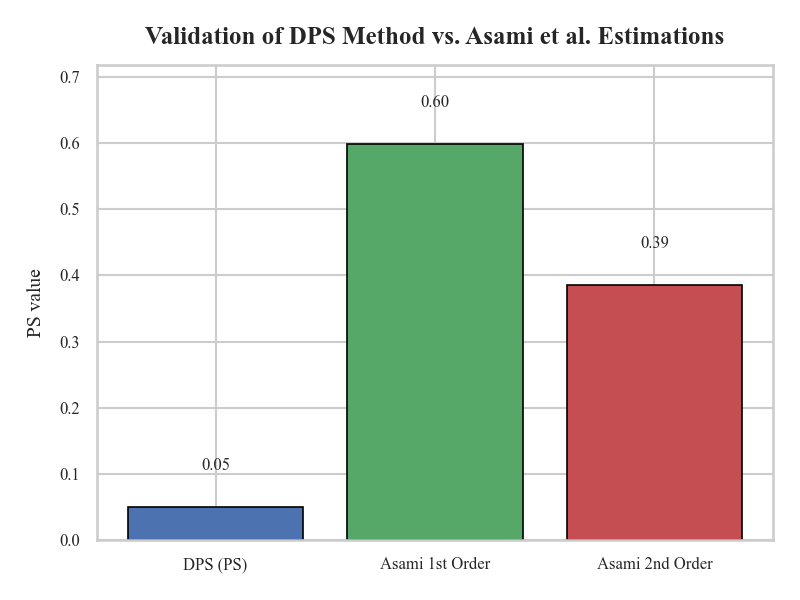
\includegraphics[width=0.5\textwidth]{picture7.png}}
\caption{مقایسه پاسخ‌های فرکانسی و معیار \lr{PS} بین روش \lr{DPS} و پاسخ‌های تحلیلی \lr{Asami}}
\label{fig:asami-frf-comparison}
\end{figure}

این نتایج تأیید می‌کنند که فرض جداسازی پارامترها در روش \lr{DPS} حتی در سیستم‌های ساده با درجات آزادی پایین نیز معتبر است. به‌عبارت دیگر، اگر روش در چنین شرایطی عملکرد دقیق داشته باشد، می‌توان انتظار داشت در سیستم‌های پیچیده‌تر با درجات آزادی بالا نیز به‌خوبی عمل کند. نکته کلیدی این است که فرآیند بهینه‌سازی در \lr{DPS} تنها بر اساس کمینه‌سازی جمع توابع جانشین از پیش محاسبه‌شده انجام می‌گیرد، بدون نیاز به شبیه‌سازی‌های تکراری سیستم کامل. این ویژگی فرآیند سنتی و پرهزینه تنظیم جاذب‌ها را به یک فرایند ساختارمند، تکرارپذیر و کم‌هزینه تبدیل می‌کند.

در نهایت، با امکان استفاده مستقیم از این توابع جانشین در معماری‌های مختلف سیستم، چارچوب \lr{DPS} بستری برای توسعه کاتالوگ‌های طراحی فراهم می‌آورد که نیاز به بهینه‌سازی‌های عددی مجدد را حذف کرده و انتخاب سریع پارامترهای نزدیک به بهینه را برای مهندسان ممکن می‌سازد.

% --- پایان بخش ---
% -----------------------------
% Section: Generalized Optimization with DPS-Derived Catalogues
% -----------------------------

\section{بهینه‌سازی تعمیم‌یافته با استفاده از کاتالوگ‌های مشتق‌شده از چارچوب \lr{DPS}}

پس از اعتبارسنجی موفق چارچوب \lr{DPS}، در این بخش الگوریتمی ساختاریافته برای تولید کاتالوگ‌های طراحی معرفی می‌شود که امکان بهینه‌سازی سریع پارامترهای جاذب دینامیکی ارتعاش را برای مجموعه‌ای گسترده از سیستم‌های مکانیکی فراهم می‌سازد. این قابلیت حتی برای سیستم‌هایی که تنها زیرمجموعه‌ای ساده‌شده از مدل مرجع کوپله‌شده کامل هستند نیز کاربرد دارد. اصل بنیادی چارچوب \lr{DPS} در جداسازی فضای بهینه‌سازی نهفته است؛ بدین‌گونه که هر پارامتر جاذب به تابع جانشین تک‌متغیره مستقل خود وابسته است که از مدل دینامیکیِ کامل استخراج شده است.

این رویکرد به‌گونه‌ای طراحی شده است که معادلات جداسازی‌شده حاصل، قابلیت اعمال عمومی داشته باشند و در هر پیکربندی سیستمی که درون دامنه‌های پارامترِیِ مدل‌سازی‌شده قرار گیرد، قابل استفاده باشند؛ حتی در صورتی که بعضی اجزای سیستم کامل در پیکربندی موردنظر وجود نداشته باشند. منطقِ الگوریتم جداسازی این امکان را فراهم می‌کند که چنانچه یک سامانه فاقد برخی مؤلفه‌ها باشد (برای مثال، بدون المان \lr{Inerter} یا با مقدار میراییِ قفل‌شده)، پارامتر مربوطه یا مقدار صفر در نظر گرفته شود (در صورت نبود) و یا به‌عنوان مقدار ثابت جای‌گذاری شود (در صورت قفل بودن). با این‌حال، حتی اگر مقدار یک پارامتر صفر باشد، تابع جانشین مربوطه باید همچنان در فرآیند بهینه‌سازی ارزیابی شود تا اثرات پسماند ناشی از مدل کامل در پیکربندی کاهش‌یافته نیز لحاظ گردد.

هدف بهینه‌سازی در این الگوریتم به‌صورت کمینه‌سازی مجموع تمام توابع جانشینِ جداسازی‌شده تعریف می‌شود، صرف‌نظر از این‌که پارامتر متناظر در سیستم حضور داشته باشد یا خیر. در این فرمول‌بندی، مجموعه بهینه پارامترهای جاذب زمانی حاصل می‌شود که مجموع این توابع به حداقل برسد؛ بدین معنا که نوسان بین قله‌های پاسخ به کمترین میزان رسیده و جذب ارتعاش در حالت بهینه صورت گرفته است:

\begin{equation}
\min_{\{p_i\}} \; \sum_{i=1}^{n} X_i\bigl(p_i\bigr)
\end{equation}

در این‌جا \(n\) تعداد کل توابعِ جداسازی‌شده استخراج‌شده از مدل کامل است (حتی پارامترهای غیرفعال یا صفر را شامل می‌شود).

به‌منظور پشتیبانی از این رویکرد الگوریتمی، یک کاتالوگ طراحی بر اساس چهار پیکربندی ساختاریِ متفاوت از مدل مرجع توسعه داده شد. هر پیکربندی با مجموعه‌ای مشخص از ویژگی‌های ساختاریِ ثابت مانند فرکانس طبیعی، نسبت میرایی و نسبت جرم مشخص می‌شود. برای هر پیکربندی، ده تابع جانشینِ جداسازی‌شده تولید گردید که هرکدام نمایانگر تأثیر یک پارامتر خاص از جاذب ارتعاش هستند. این توابع جانشین به‌صورت چندجمله‌ایِ درجه چهارم مدل‌سازی شده‌اند:

\begin{equation}
X_i(p_i) 
  = a_{i,0} + a_{i,1} p_i + a_{i,2} p_i^{2} + a_{i,3} p_i^{3} + a_{i,4} p_i^{4}
\end{equation}

ضرایب چندجمله‌ای \(a_{i,k}\) برای هر تابع، به‌همراه ویژگی‌های ساختاریِ هر مورد، در جدول~\ref{tab:structural-params} و جداول ضرایبِ بعدی ارائه شده‌اند.

% --------------------------------------------------------
% Structural parameters of the four reference systems
% --------------------------------------------------------

\begin{table}[ht]
  \centering
  \caption{پارامترهای ساختاری چهار سیستم مرجع}
  \label{tab:structural-params}
  \begin{tabular}{c c c c c c c}
    \hline
    \lr{System} & $\Lambda$ & $N$ & $A_{Up}{=}A_{Low}$ & $F$ & $\omega_{dc}$ & $\zeta_{dc}$ \\
    \hline
    \lr{1} & \lr{1.00} & \lr{1.00} & \lr{1e-4} & \lr{100} & \lr{1000} & \lr{0.01} \\
    \lr{2} & \lr{0.75} & \lr{0.75} & \lr{1e-4} & \lr{100} & \lr{800}  & \lr{0.02} \\
    \lr{3} & \lr{0.50} & \lr{0.50} & \lr{1e-4} & \lr{100} & \lr{800}  & \lr{0.02} \\
    \lr{4} & \lr{0.50} & \lr{0.50} & \lr{1e-4} & \lr{100} & \lr{700}  & \lr{0.03} \\
    \hline
  \end{tabular}
\end{table}

\bigskip

% --------------------------------------------------------
% Polynomial coefficients tables (Systems 1--4)
% --------------------------------------------------------

% ---------- System 1 ----------
\begin{table}[ht]
  \centering
  \scriptsize
  \caption{ضرایب چندجمله‌ای چارچوب \protect\lr{DPS} برای سیستم \protect\lr{1}}
  \label{tab:dps-coeff-sys1}
  \begin{tabular}{l r r r r r}
    \hline
      & $a_{4}$ & $a_{3}$ & $a_{2}$ & $a_{1}$ & $a_{0}$ \\
    \hline
    $\mu_{1}$     & \lr{$-8.2269e-12$} & \lr{$2.2743e-10$} & \lr{$-2.1919e-09$} & \lr{$8.5432e-09$}  & \lr{$-1.1436e-08$} \\
    $\beta_{1}$   & \lr{$1.2785e-11$}  & \lr{$-2.9913e-10$} & \lr{$2.6576e-09$}  & \lr{$-8.3011e-09$} & \lr{$-2.7080e-09$} \\
    $\lambda_{1}$ & \lr{$3.3333e-12$}  & \lr{$-1.1461e-10$} & \lr{$6.9518e-10$}  & \lr{$-2.7359e-10$} & \lr{$1.1169e-09$} \\
    $\nu_{1}$     & \lr{$3.4793e-12$}  & \lr{$-7.5003e-11$} & \lr{$5.1341e-10$}  & \lr{$-2.7621e-09$} & \lr{$1.5231e-08$} \\
    $\beta_{7}$   & \lr{$4.3369e-11$}  & \lr{$-9.1300e-10$} & \lr{$5.6815e-09$}  & \lr{$-1.1223e-08$} & \lr{$2.5909e-08$} \\
    $\lambda_{7}$ & \lr{$-4.6563e-11$} & \lr{$9.9032e-10$}  & \lr{$-6.4370e-09$} & \lr{$1.3672e-08$}  & \lr{$-2.7614e-08$} \\
    $\nu_{7}$     & \lr{$-3.1186e-12$} & \lr{$8.3988e-11$}  & \lr{$-5.1866e-10$} & \lr{$9.5108e-10$}  & \lr{$-1.3858e-10$} \\
    $\beta_{8}$   & \lr{$-3.0277e-11$} & \lr{$1.1787e-09$}  & \lr{$-1.5057e-08$} & \lr{$6.9366e-08$}  & \lr{$-6.3326e-08$} \\
    $\lambda_{8}$ & \lr{$2.4785e-11$}  & \lr{$-1.0481e-09$} & \lr{$1.3963e-08$}  & \lr{$-6.5790e-08$} & \lr{$6.0165e-08$} \\
    $\nu_{8}$     & \lr{$1.7830e-13$}  & \lr{$-2.1887e-11$} & \lr{$5.8945e-10$}  & \lr{$-4.1231e-09$} & \lr{$4.9205e-09$} \\
    \hline
  \end{tabular}
\end{table}

% ---------- System 2 ----------
\begin{table}[ht]
  \centering
  \scriptsize
  \caption{ضرایب چندجمله‌ای چارچوب \protect\lr{DPS} برای سیستم \protect\lr{2}}
  \label{tab:dps-coeff-sys2}
  \begin{tabular}{l r r r r r}
    \hline
      & $a_{4}$ & $a_{3}$ & $a_{2}$ & $a_{1}$ & $a_{0}$ \\
    \hline
    $\mu_{1}$     & \lr{$-4.2169e-12$} & \lr{$1.2141e-10$}  & \lr{$-1.2323e-09$} & \lr{$5.5550e-09$}  & \lr{$-1.1764e-08$} \\
    $\beta_{1}$   & \lr{$1.0636e-11$}  & \lr{$-2.3902e-10$} & \lr{$1.9574e-09$}  & \lr{$-5.1823e-09$} & \lr{$-2.0384e-09$} \\
    $\lambda_{1}$ & \lr{$4.8080e-13$}  & \lr{$-4.7496e-11$} & \lr{$2.8672e-10$}  & \lr{$6.2064e-11$}  & \lr{$-5.8066e-10$} \\
    $\nu_{1}$     & \lr{$1.3318e-13$}  & \lr{$1.4513e-11$}  & \lr{$-3.3418e-10$} & \lr{$4.6261e-10$}  & \lr{$1.1578e-08$} \\
    $\beta_{7}$   & \lr{$6.1234e-11$}  & \lr{$-1.2616e-09$} & \lr{$7.7004e-09$}  & \lr{$-1.4060e-08$} & \lr{$2.3311e-08$} \\
    $\lambda_{7}$ & \lr{$-6.3736e-11$} & \lr{$1.3240e-09$}  & \lr{$-8.3711e-09$} & \lr{$1.6329e-08$}  & \lr{$-2.4919e-08$} \\
    $\nu_{7}$     & \lr{$-3.4698e-12$} & \lr{$9.3584e-11$}  & \lr{$-5.9060e-10$} & \lr{$1.1988e-09$}  & \lr{$-3.8190e-10$} \\
    $\beta_{8}$   & \lr{$1.4112e-12$}  & \lr{$4.8618e-10$}  & \lr{$-1.0332e-08$} & \lr{$6.0675e-08$}  & \lr{$-7.2392e-08$} \\
    $\lambda_{8}$ & \lr{$-3.6533e-12$} & \lr{$-4.3901e-10$} & \lr{$9.9743e-09$}  & \lr{$-5.9718e-08$} & \lr{$7.2568e-08$} \\
    $\nu_{8}$     & \lr{$8.7218e-13$}  & \lr{$-4.2572e-11$} & \lr{$8.3451e-10$}  & \lr{$-5.3544e-09$} & \lr{$6.7529e-09$} \\
    \hline
  \end{tabular}
\end{table}

% ---------- System 3 ----------
\begin{table}[ht]
  \centering
  \scriptsize
  \caption{ضرایب چندجمله‌ای چارچوب \protect\lr{DPS} برای سیستم \protect\lr{3}}
  \label{tab:dps-coeff-sys3}
  \begin{tabular}{l r r r r r}
    \hline
      & $a_{4}$ & $a_{3}$ & $a_{2}$ & $a_{1}$ & $a_{0}$ \\
    \hline
    $\mu_{1}$     & \lr{$-4.1081e-12$} & \lr{$1.1424e-10$}  & \lr{$-1.1141e-09$} & \lr{$4.9374e-09$}  & \lr{$-1.1596e-08$} \\
    $\beta_{1}$   & \lr{$1.2882e-11$}  & \lr{$-2.8725e-10$} & \lr{$2.1328e-09$}  & \lr{$-4.1703e-09$} & \lr{$-3.1410e-09$} \\
    $\lambda_{1}$ & \lr{$-1.3282e-12$} & \lr{$8.7284e-12$}  & \lr{$-2.0724e-10$} & \lr{$1.2659e-09$}  & \lr{$-2.3467e-09$} \\
    $\nu_{1}$     & \lr{$-3.0662e-13$} & \lr{$2.7309e-11$}  & \lr{$-4.3590e-10$} & \lr{$4.8020e-10$}  & \lr{$1.3097e-08$} \\
    $\beta_{7}$   & \lr{$5.5906e-11$}  & \lr{$-1.0275e-09$} & \lr{$4.6508e-09$}  & \lr{$-2.4566e-10$} & \lr{$9.8006e-09$} \\
    $\lambda_{7}$ & \lr{$-5.9476e-11$} & \lr{$1.1141e-09$}  & \lr{$-5.5237e-09$} & \lr{$3.0669e-09$}  & \lr{$-1.1962e-08$} \\
    $\nu_{7}$     & \lr{$-3.7642e-12$} & \lr{$9.6193e-11$}  & \lr{$-5.2460e-10$} & \lr{$6.3498e-10$}  & \lr{$5.4645e-10$} \\
    $\beta_{8}$   & \lr{$-2.6076e-11$} & \lr{$1.3459e-09$}  & \lr{$-1.9714e-08$} & \lr{$1.0138e-07$}  & \lr{$-1.2572e-07$} \\
    $\lambda_{8}$ & \lr{$2.4964e-11$}  & \lr{$-1.3287e-09$} & \lr{$1.9607e-08$}  & \lr{$-1.0115e-07$} & \lr{$1.2625e-07$} \\
    $\nu_{8}$     & \lr{$8.9637e-13$}  & \lr{$-5.0816e-11$} & \lr{$1.0127e-09$}  & \lr{$-6.3609e-09$} & \lr{$7.4244e-09$} \\
    \hline
  \end{tabular}
\end{table}

% ---------- System 4 ----------
\begin{table}[ht]
  \centering
  \scriptsize
  \caption{ضرایب چندجمله‌ای چارچوب \protect\lr{DPS} برای سیستم \protect\lr{4}}
  \label{tab:dps-coeff-sys4}
  \begin{tabular}{l r r r r r}
    \hline
      & $a_{4}$ & $a_{3}$ & $a_{2}$ & $a_{1}$ & $a_{0}$ \\
    \hline
    $\mu_{1}$     & \lr{$1.0580e-11$}  & \lr{$-3.3315e-10$} & \lr{$3.8848e-09$}  & \lr{$-1.9060e-08$} & \lr{$2.9010e-08$} \\
    $\beta_{1}$   & \lr{$6.9658e-12$}  & \lr{$-1.2374e-10$} & \lr{$5.0191e-10$}  & \lr{$2.2950e-09$}  & \lr{$-9.1548e-09$} \\
    $\lambda_{1}$ & \lr{$-1.1743e-11$} & \lr{$3.0699e-10$}  & \lr{$-3.3189e-09$} & \lr{$1.5790e-08$}  & \lr{$-3.0429e-08$} \\
    $\nu_{1}$     & \lr{$2.4462e-12$}  & \lr{$-5.2918e-11$} & \lr{$4.2835e-10$}  & \lr{$-3.7223e-09$} & \lr{$2.1408e-08$} \\
    $\beta_{7}$   & \lr{$-2.4987e-11$} & \lr{$6.6586e-10$}  & \lr{$-4.7916e-09$} & \lr{$-4.3244e-09$} & \lr{$1.0973e-07$} \\
    $\lambda_{7}$ & \lr{$8.3603e-13$}  & \lr{$7.0632e-11$}  & \lr{$-3.6724e-09$} & \lr{$4.5886e-08$}  & \lr{$-1.8443e-07$} \\
    $\nu_{7}$     & \lr{$-2.6664e-12$} & \lr{$6.3649e-11$}  & \lr{$-1.6792e-10$} & \lr{$-1.0670e-09$} & \lr{$3.5905e-09$} \\
    $\beta_{8}$   & \lr{$4.9277e-11$}  & \lr{$-1.9031e-09$} & \lr{$2.8576e-08$}  & \lr{$-1.9746e-07$} & \lr{$5.2849e-07$} \\
    $\lambda_{8}$ & \lr{$-4.0292e-11$} & \lr{$1.6182e-09$}  & \lr{$-2.5352e-08$} & \lr{$1.8158e-07$}  & \lr{$-4.9873e-07$} \\
    $\nu_{8}$     & \lr{$9.2586e-12$}  & \lr{$-3.0220e-10$} & \lr{$3.8118e-09$}  & \lr{$-2.0104e-08$} & \lr{$3.2698e-08$} \\
    \hline
  \end{tabular}
\end{table}

\bigskip

% --------------------------------------------------------
% Frequency response figure
% --------------------------------------------------------
\begin{figure}[ht]
  \centering
  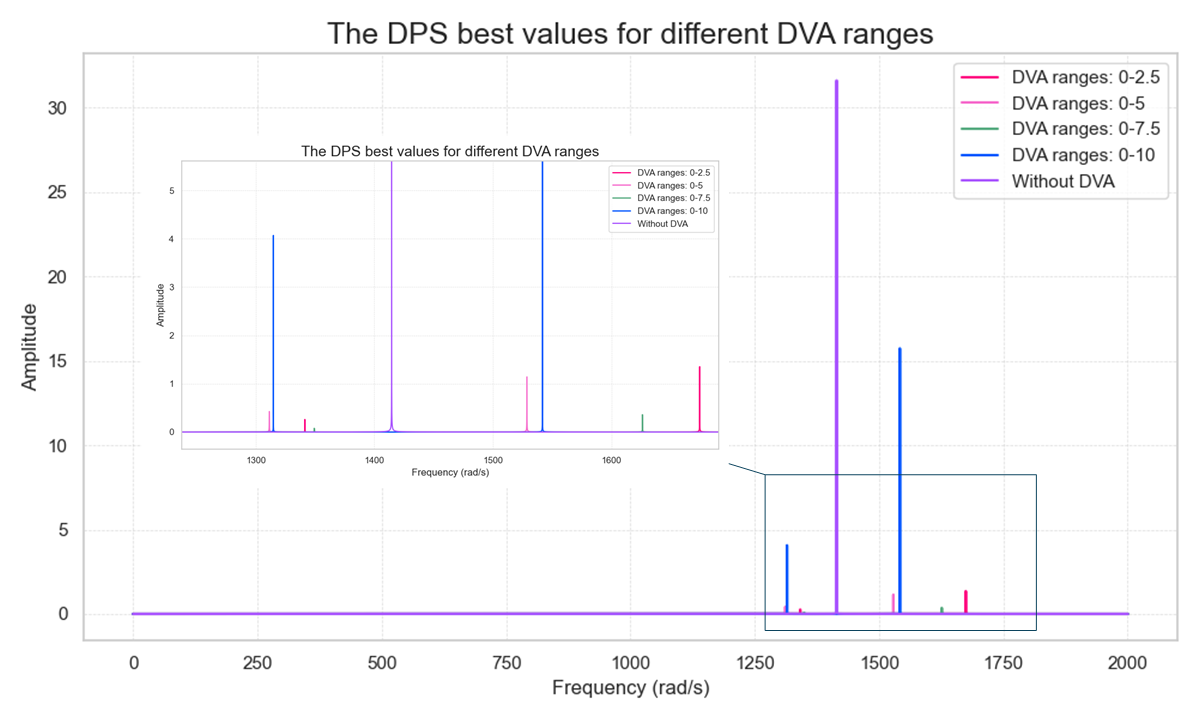
\includegraphics[width=0.9\linewidth]{picture9.png}
  \caption{توابع پاسخ فرکانسی (\lr{FRF}) سیستم \protect\lr{1} پس از بهینه‌سازی با روش \protect\lr{DPS} در بازه‌های پارامتری مختلف.}
  \label{fig:frf-system1}
\end{figure}

% --------------------------------------------------------
% Catalogue usage guide
% --------------------------------------------------------

\subsubsection*{راهنمای استفاده از کاتالوگ}

\begin{enumerate}
  \item \textbf{شناسایی پارامترهای موجود:} ابتدا پارامترهای جاذبِ حاضر در سیستم تعیین و مقادیر غایب برابر صفر فرض می‌شوند.
  \item \textbf{اعمال قیود ثابت:} در صورت وجود پارامترهای ثابت (به‌دلایل طراحی یا محدودیت‌های فیزیکی)، مقادیرشان در توابع جانشین جای‌گذاری می‌شود.
  \item \textbf{ساخت توابع جانشین:} برای هر پارامتر آزاد، ضرایبِ چندجمله‌ای از کاتالوگ استخراج، و تابع $X_i(p_i)$ ساخته می‌شود.
  \item \textbf{بهینه‌سازی:} با کمینه‌سازی مجموع $\sum_i X_i(p_i)$ برحسب متغیرهای آزاد، مقادیر بهینه پارامترها به دست می‌آید.
  \item \textbf{استخراج نتایج:} بردار پارامترهای جاذب که کمترین مقدار را برای مجموع \lr{DPS} ایجاد می‌کند، به‌عنوان پاسخِ بهینه در نظر گرفته می‌شود.
\end{enumerate}

مطابق تحلیل حساسیت ارائه‌شده در پیوست «الف»، چارچوب جانشین پیشنهادی حتی تحت تغییرات ملایمِ پارامترهای سازه‌ای نیز دقت مطلوبی حفظ می‌کند؛ موضوعی که مسیر توسعه به یک کاتالوگ جامع‌تر با دربرگیری همزمان متغیرهای سازه‌ای و جاذب را هموار می‌سازد.

% -----------------------------
% End of Section
% -----------------------------


\section{کاتالوگ تعمیم‌یافته مبتنی بر \lr{DPS} و تحلیل حساسیت سازه‌ای}

هدف این بخش، یکپارچه‌سازی منطق کاتالوگ‌های طراحی مشتق‌شده از چارچوب 
\lr{DPS}
 با ارزیابی حدود اعتبار آن در برابر تغییرات پارامترهای سازه‌ای است. ایده محوری 
 \lr{DPS}
  بر جداسازی فضای بهینه‌سازی است: هر پارامتر جاذب دینامیکی ارتعاش 
  \lr{DVA}
   به یک تابع جانشین تک‌متغیره نگاشت می‌شود که از مدل ‌کاملا کوپل شده استخراج می شود. چنین جداسازی‌ای اجازه می‌دهد معادلات حاصل، برای هر سیستمی که در بازه‌های پارامتری مدل‌سازی‌شده قرار دارد، به‌صورت عمومی به‌کار روند اگر برخی مؤلفه‌های مدل کامل (مانند المان 
   \lr{Inerter})
    غایب باشند یا مقادیری ثابت داشته باشند. در این حالت، پارامتر متناظر یا صفر گذاشته می‌شود (در صورت نبود) یا به‌صورت ثابت جایگذاری می‌گردد. با این وجود، تابع جانشین مربوط به هر پارامتر اگر مقدارش صفر باشد باید همچنان ارزیابی و در جمع کل لحاظ شود تا اثرات پسماند مدل مرجع به‌درستی منعکس گردد. معیار بهینه‌سازی، کمینه‌سازی مجموع تمام توابع جانشین جداسازی‌شده است و پاسخ بهینه زمانی حاصل می‌شود که این مجموع به نزدیک صفر میل کند و بدین‌ترتیب اختلاف قله‌ها در 
    \lr{FRF}
     حداقل شود.

\subsection{دامنه و محدودیت‌ها}
در این فصل، تغییرات ضرایب جانشین نسبت به پارامترهای سازه‌ای مطالعه نشده است. تعمیم کاتالوگ به حالتی که هم تنوع سازه و هم تنظیم‌پذیری جاذب را دربرگیرد، مستلزم گسترش فضای پارامتر، طراحی طرح‌نمونه‌برداری جدید، و احتمالاً استفاده از خانواده‌های متفاوتی از مدل‌های جانشین است. به‌منظور حفظ شفافیت دامنه و تمرکز بر اعتبارسنجی جداسازی «فقط-جاذب» در مقایسه با الگوریتم‌های ژنتیک تمام‌کوپله، این مسیر عمداً از حیطه کار خارج شده است. برای مواجهه جزئی با این محدودیت، تحلیلی از حساسیت نسبت به پارامترهای سازه‌ای در ضمیمه \lr{A} ارائه شده است—در حالی‌که پارامترهای جاذب ثابت نگاه داشته می‌شوند—و خطای نسبی بین 
\lr{DPS}
 مبتنی بر جانشین و 
 \lr{PS}
  مدل کامل، بر روی بازه‌ای واقع‌گرایانه گزارش می‌گردد. هم‌خوانی قوی مشاهده‌شده، نشان می‌دهد که مدل جانشین تحت تغییرات سازه‌ای «میانه» همچنان دقیق باقی می‌ماند و از این رو، انگیزه‌ای برای توسعه چارچوب‌های تعمیم‌یافته‌تر (شامل سازه) فراهم می‌کند.

\subsection{روش تحلیل حساسیت سازه‌ای با \lr{DVA} ثابت}
در تحلیل حساسیت، اثر تغییرات پارامترهای سامانه اصلی در حالی بررسی می‌شود که مقادیر 
\lr{DVA}
 ثابت هستند. هدف، درک وابستگی 
 \lr{DPS}
  به پارامترهای سازه‌ای در پیکربندی‌هایی است که 
  \lr{DVA}
   تغییر نمی‌کند. گام‌های اجرایی به‌صورت خلاصه عبارت‌اند از:
\begin{enumerate}
  \item \textbf{تعیین مجموعه‌های ثابت 
  \lr{DVA}:}
   چند مجموعه بعددار از پارامترهای جاذب انتخاب و ثابت می‌شوند تا رفتار 
   \lr{DPS}
    تنها نسبت به تغییرات سازه‌ای سنجیده شود.
  \item \textbf{پوشش بازه‌های سازه‌ای:} برای هر پارامتر سازه‌ای، پیمایش گسترده در محدوده‌های از پیش تعیین‌شده انجام می‌گیرد تا اثر آن بر 
  \lr{DPS}
   روی طیف وسیعی از حالات آشکار شود.
  \item \textbf{محاسبه شاخص خطای نسبی:} خطای نسبی بین 
  \lr{PS}
   مدل کامل و 
   \lr{DPS}
    جانشین به‌عنوان معیار عملکرد اصلی محاسبه می‌شود. تعریف متعارفِ مورد استفاده:
  \begin{equation}
    \varepsilon_{\mathrm{rel}} \;=\; \frac{\bigl|\mathrm{PS}_{\mathrm{full}} - \mathrm{PS}_{\mathrm{DPS}}\bigr|}{\mathrm{PS}_{\mathrm{full}}} \times 100\,\%.
  \end{equation}
  \item \textbf{گزارش و تفکیک‌پذیری:} نتایج به تفکیک پارامترهای سازه‌ای و برای مجموعه‌های مختلف 
  \lr{DVA}
   نمایش داده می‌شوند تا الگوهای حساسیت به‌روشنی قابل مشاهده باشند.
\end{enumerate}

\subsection{شاخص‌ها و نمادگذاری}
حساسیت نسبت به مجموعه‌ای از شاخص‌های سازه‌ای مورد بررسی قرار گرفته است؛ از جمله $A_{Low}$ و $A_{Up}$، پارامتر $F$، شمارنده مودهای مؤثر $N$، ماتریس نگاشت $\mathbf{\Lambda}$، و پارامترهای مود غالب $\mathbf{\omega}_{dc}$ و $\zeta_{dc}$. این کمیت‌ها به‌ترتیب در شکل‌های \ref{fig:ALowAUp} تا \ref{fig:zeta_ranges} (ضمیمه \lr{A}) گزارش شده‌اند:
\begin{enumerate}
  \item شکل‌های \ref{fig:ALowAUp} و\ref{fig:N_sens}: حساسیت $A_{Low}$، $A_{Up}$، $F$ و $N$ نسبت به تغییرات \lr{DVA}.
  \item شکل \ref{fig:Lambda_sens}: حساسیت $\mathbf{\Lambda}$.
  \item شکل \ref{fig:omega_dc_sens}: حساسیت $\mathbf{\omega}_{dc}$.
  \item شکل \ref{fig:zeta_ranges}: حساسیت $\zeta_{dc}$ در دو بازه (الف) $0$ تا $0.4$ و (ب) $0.4$ تا $1$.
\end{enumerate}
% --- پایان بخش ---


\subsection{نتایج و برداشت‌های کلیدی}
نتایج تحلیل حساسیت، استحکام صورت‌بندی \lr{DPS} را تأیید می‌کنند. با تغییر سیستماتیک پارامترهای سازه‌ای و ثابت نگه‌داشتن \lr{DVA}، خطای نسبی بین پیش‌بینی \lr{DPS} و پاسخ \lr{PS} مدل کامل به‌طور پیوسته پایین باقی مانده است؛ در اغلب موارد کمتر از $1\%$ و معمولاً به‌مراتب کمتر از $0.5\%$. حتی پارامترهایی که مشخصات مودال را به‌طور معنادار دگرگون می‌کنند—نظیر $\omega_{dc}$ و $\zeta_{dc}$—در بازه‌های آزموده‌شده تنها افت ناچیزی در عملکرد \lr{DPS} ایجاد کرده‌اند. این رفتار نشان می‌دهد که در حدود عملی و واقع‌گرایانه، جانشین \lr{DPS} تا حد زیادی مستقل از ریزه‌کاری‌های سازه میزبان عمل می‌کند؛ نتیجه‌ای که اعتبار استفاده ماژولار و قابل‌استفاده‌مجدد از کاتالوگ‌های طراحی مبتنی بر \lr{DPS} را تقویت می‌کند.


% شکل A.1 — تحلیل حساسیت A_Low و A_Up در برابر تغییرات پارامترهای \lr{DVA}
\begin{figure}[htbp]
  \centering
    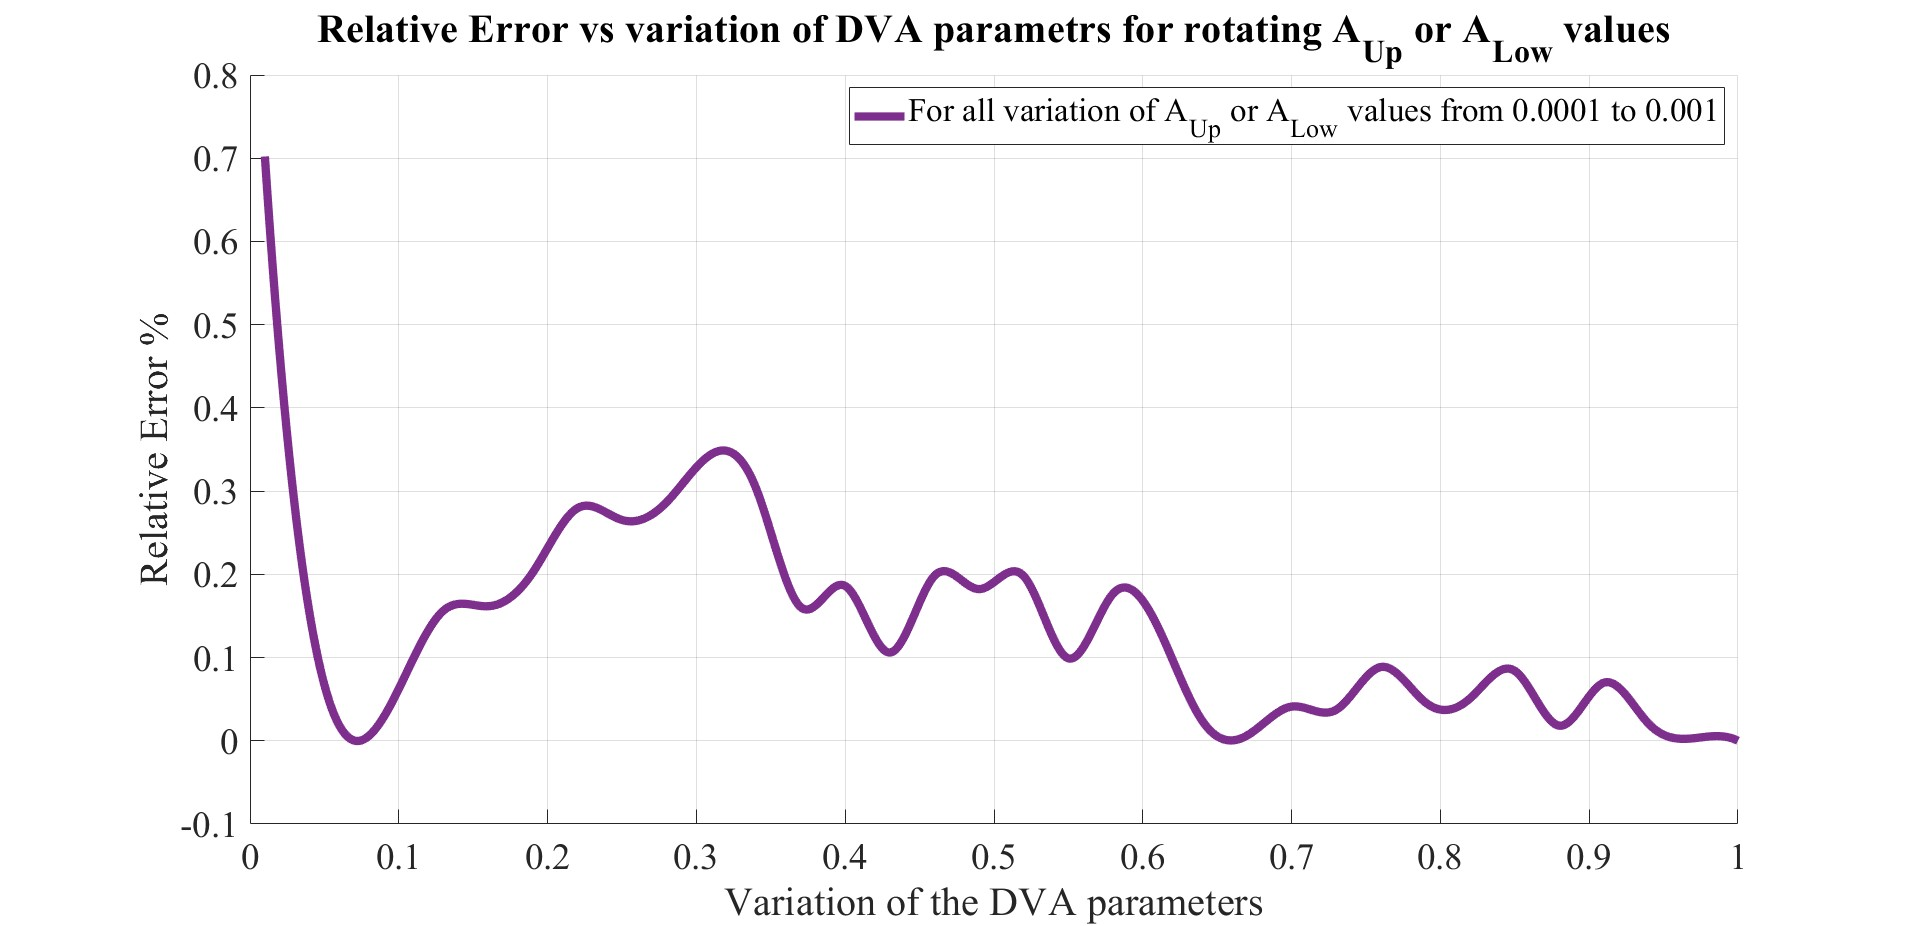
\includegraphics[width=\linewidth]{Fig.sens.Aup.jpg}
  \caption{تحلیل حساسیت $A_{\mathrm{Low}}$ و $A_{\mathrm{Up}}$ برای تغییرات مختلف پارامترهای \lr{DVA}.}
  \label{fig:ALowAUp}
\end{figure}

% شکل A.2 — تحلیل حساسیت F در برابر تغییرات پارامترهای \lr{DVA}
\begin{figure}[htbp]
  \centering
  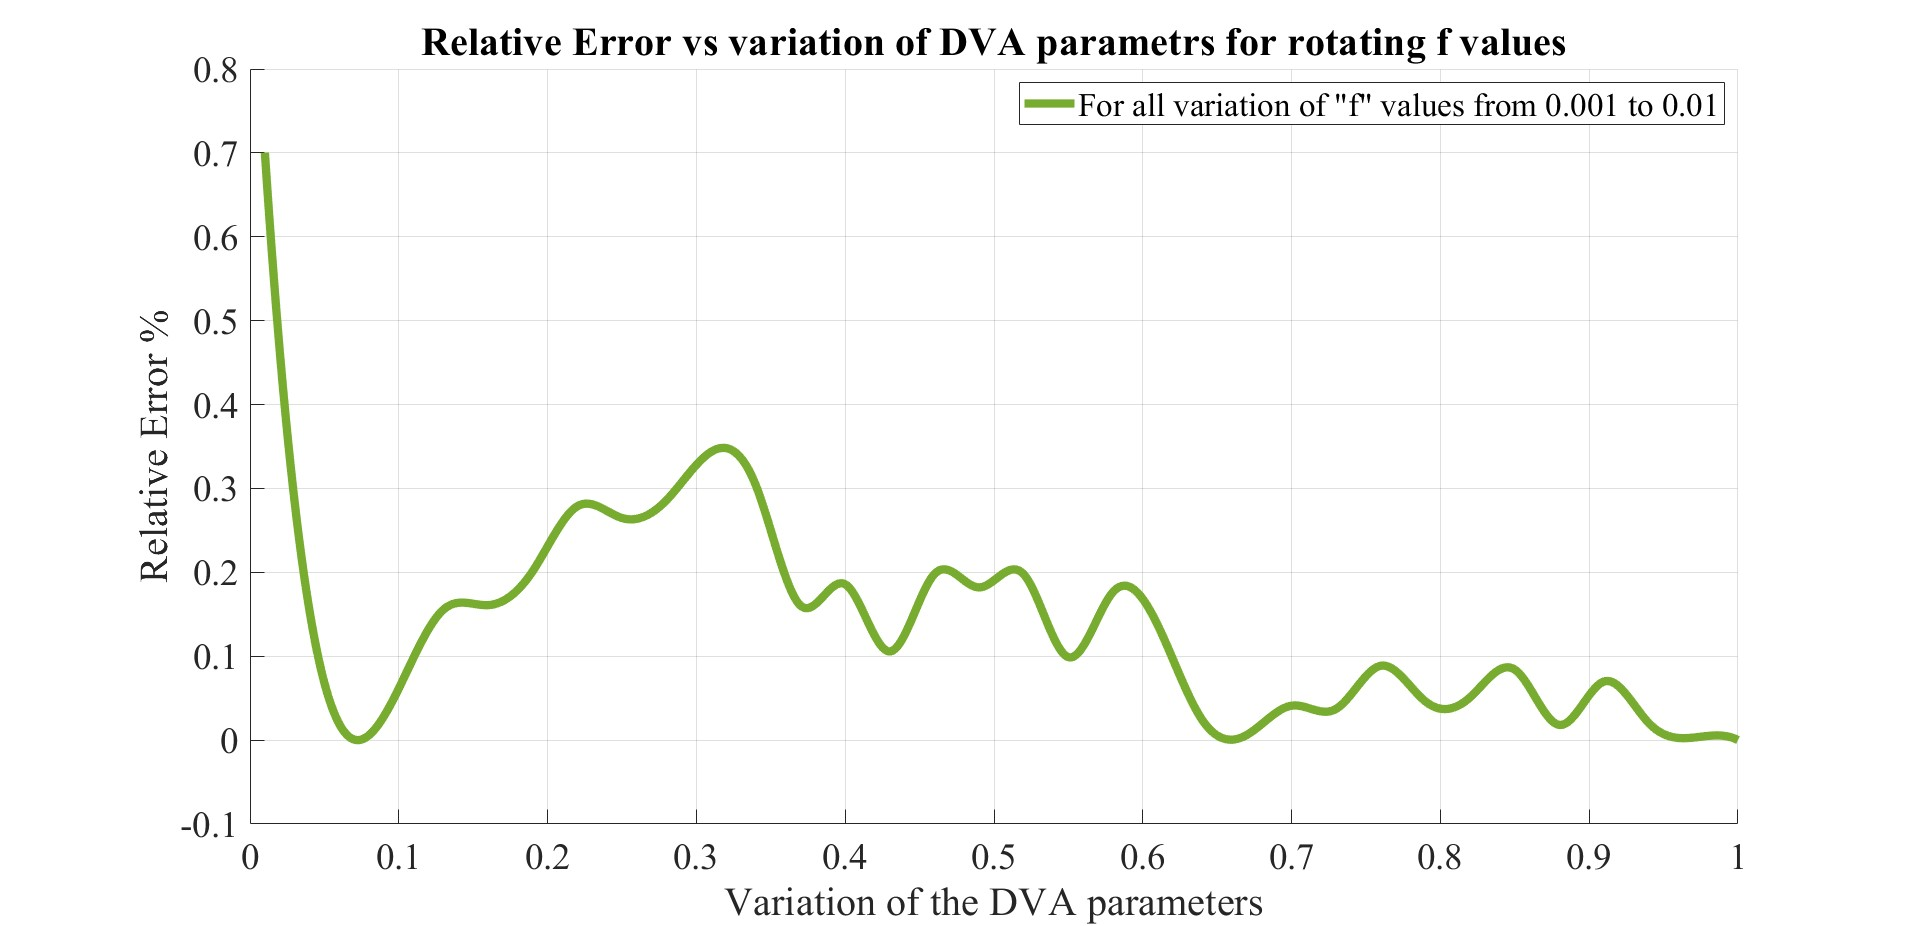
\includegraphics[width=0.8\linewidth]{Fig.sens.F.jpg}
  \caption{تحلیل حساسیت $F$ برای تغییرات مختلف پارامترهای \lr{DVA}.}
  \label{fig:F_sens}
\end{figure}

% شکل A.3 — تحلیل حساسیت N در برابر تغییرات پارامترهای \lr{DVA}
\begin{figure}[htbp]
  \centering
  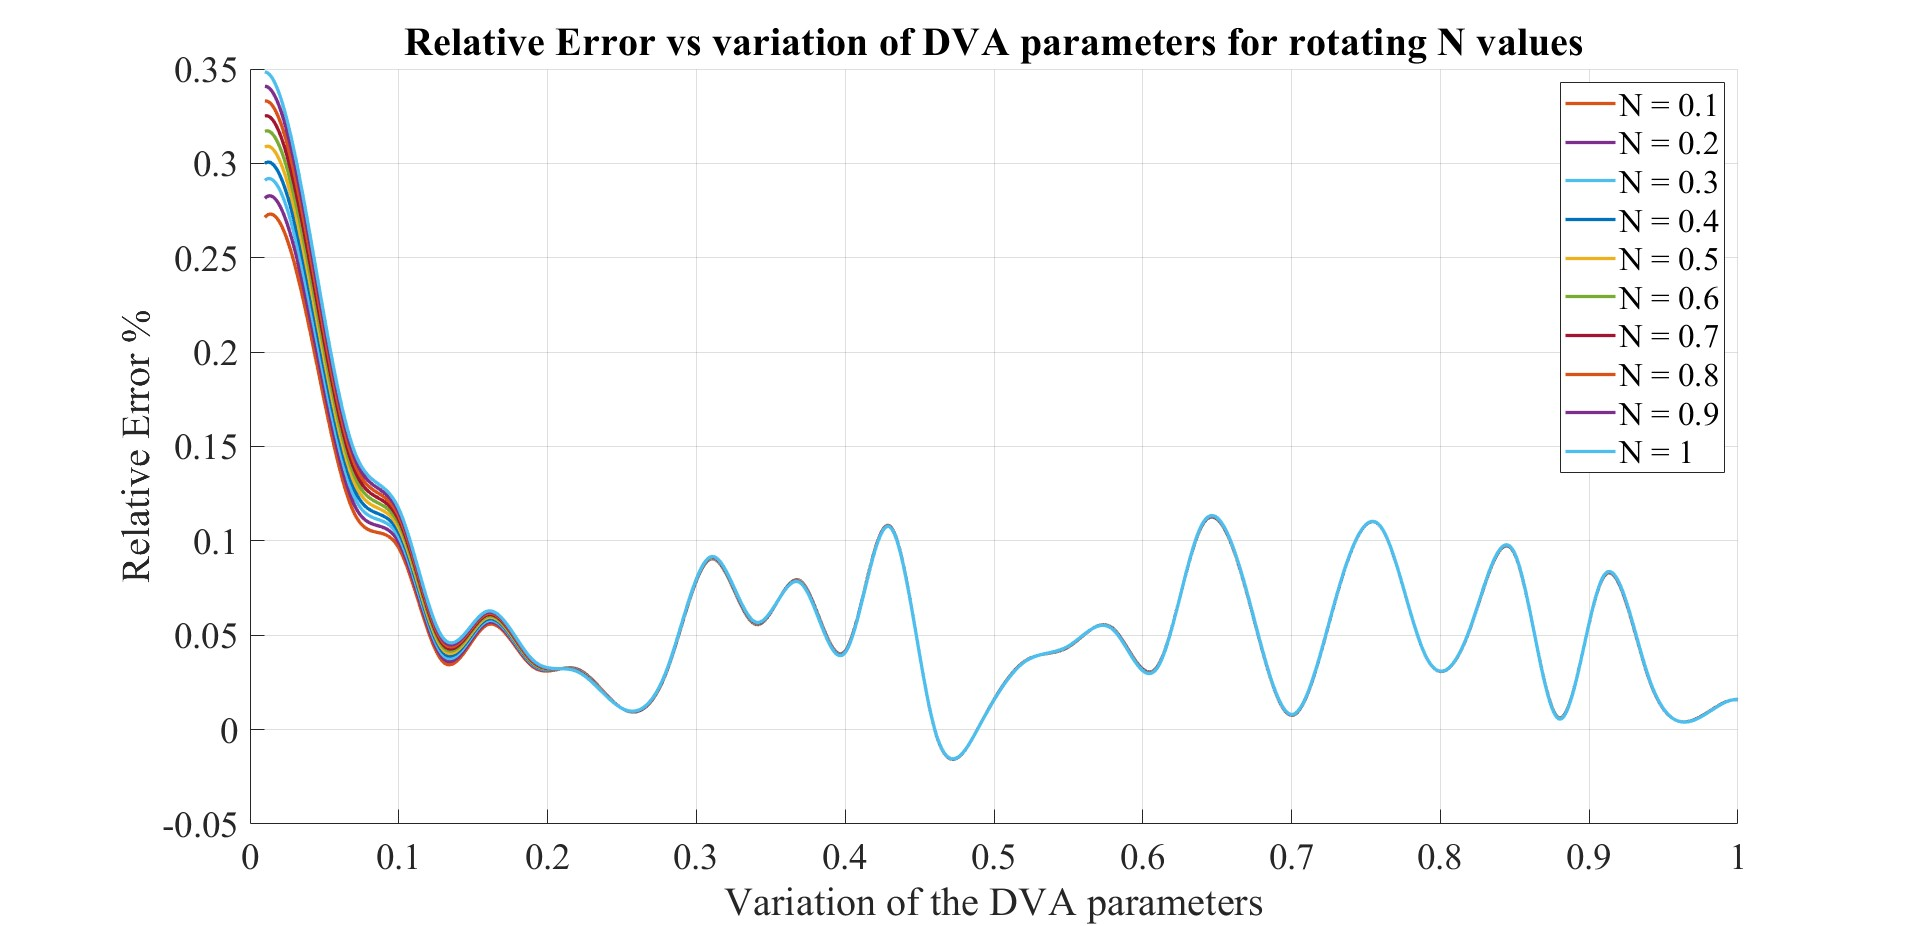
\includegraphics[width=0.8\linewidth]{Fig.sens.Nu.jpg}
  \caption{تحلیل حساسیت $N$ برای تغییرات مختلف پارامترهای \lr{DVA}.}
  \label{fig:N_sens}
\end{figure}

% شکل A.4 — تحلیل حساسیت \Lambda در برابر تغییرات پارامترهای \lr{DVA}
\begin{figure}[htbp]
  \centering
  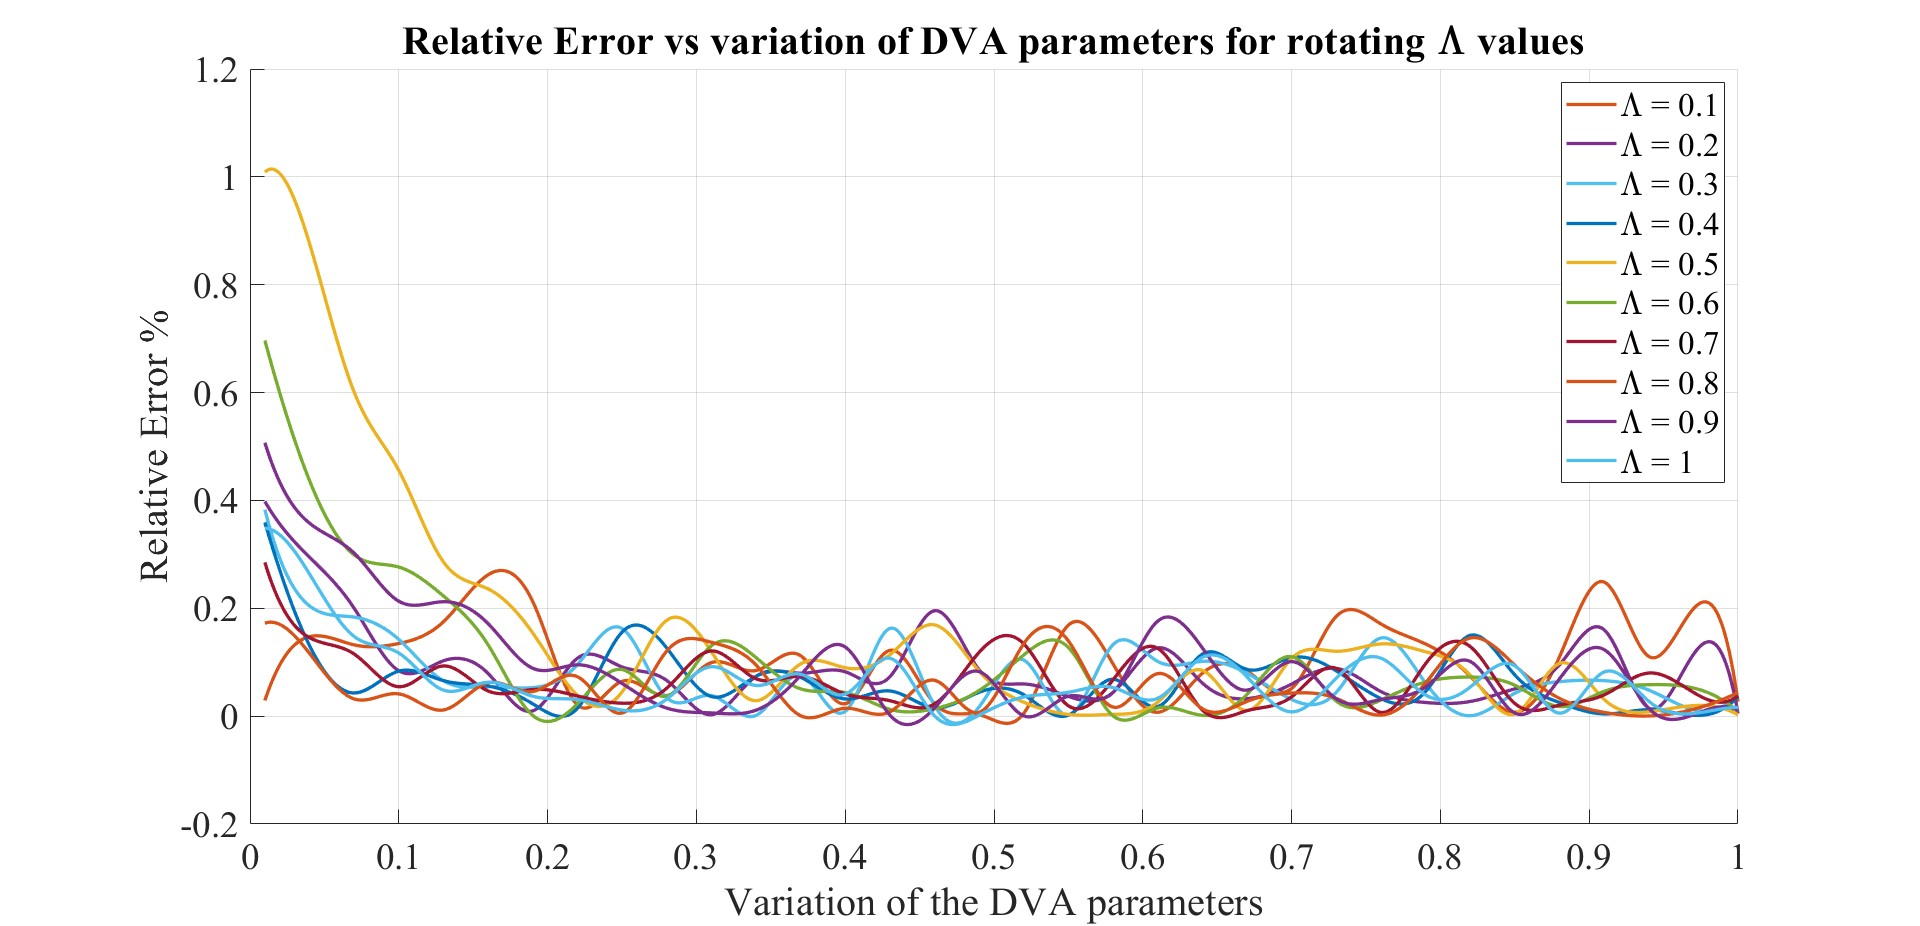
\includegraphics[width=0.8\linewidth]{Fig.sens.Lambda.jpg}
  \caption{تحلیل حساسیت $\Lambda$ برای تغییرات مختلف پارامترهای \lr{DVA}.}
  \label{fig:Lambda_sens}
\end{figure}

% شکل A.5 — تحلیل حساسیت \omega_{dc} در برابر تغییرات پارامترهای \lr{DVA}
\begin{figure}[htbp]
  \centering
  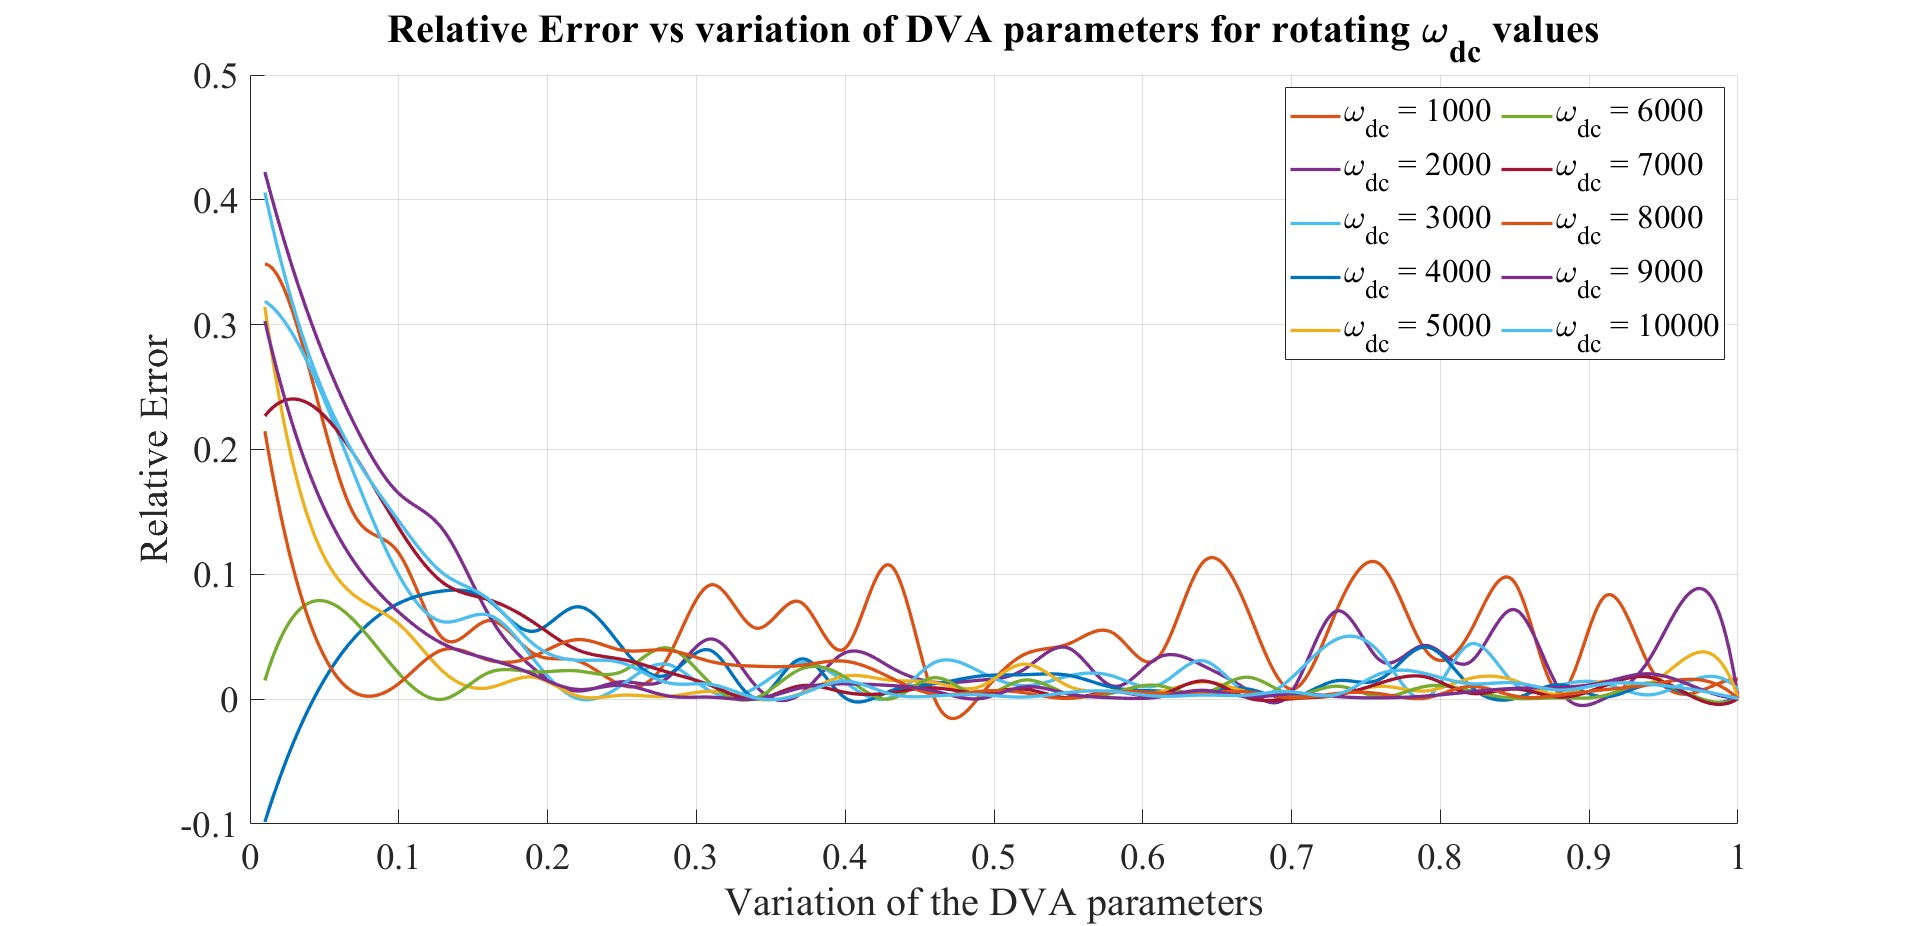
\includegraphics[width=0.8\linewidth]{Fig.sens.Omegadc.jpg}
  \caption{تحلیل حساسیت $\omega_{dc}$ برای تغییرات مختلف پارامترهای \lr{DVA}.}
  \label{fig:omega_dc_sens}
\end{figure}

% شکل A.6 — تحلیل حساسیت \zeta_{dc} در دو بازه (a) و (b)
\begin{figure}[htbp]
  \centering
  \begin{subfigure}[t]{\linewidth}
    \centering
    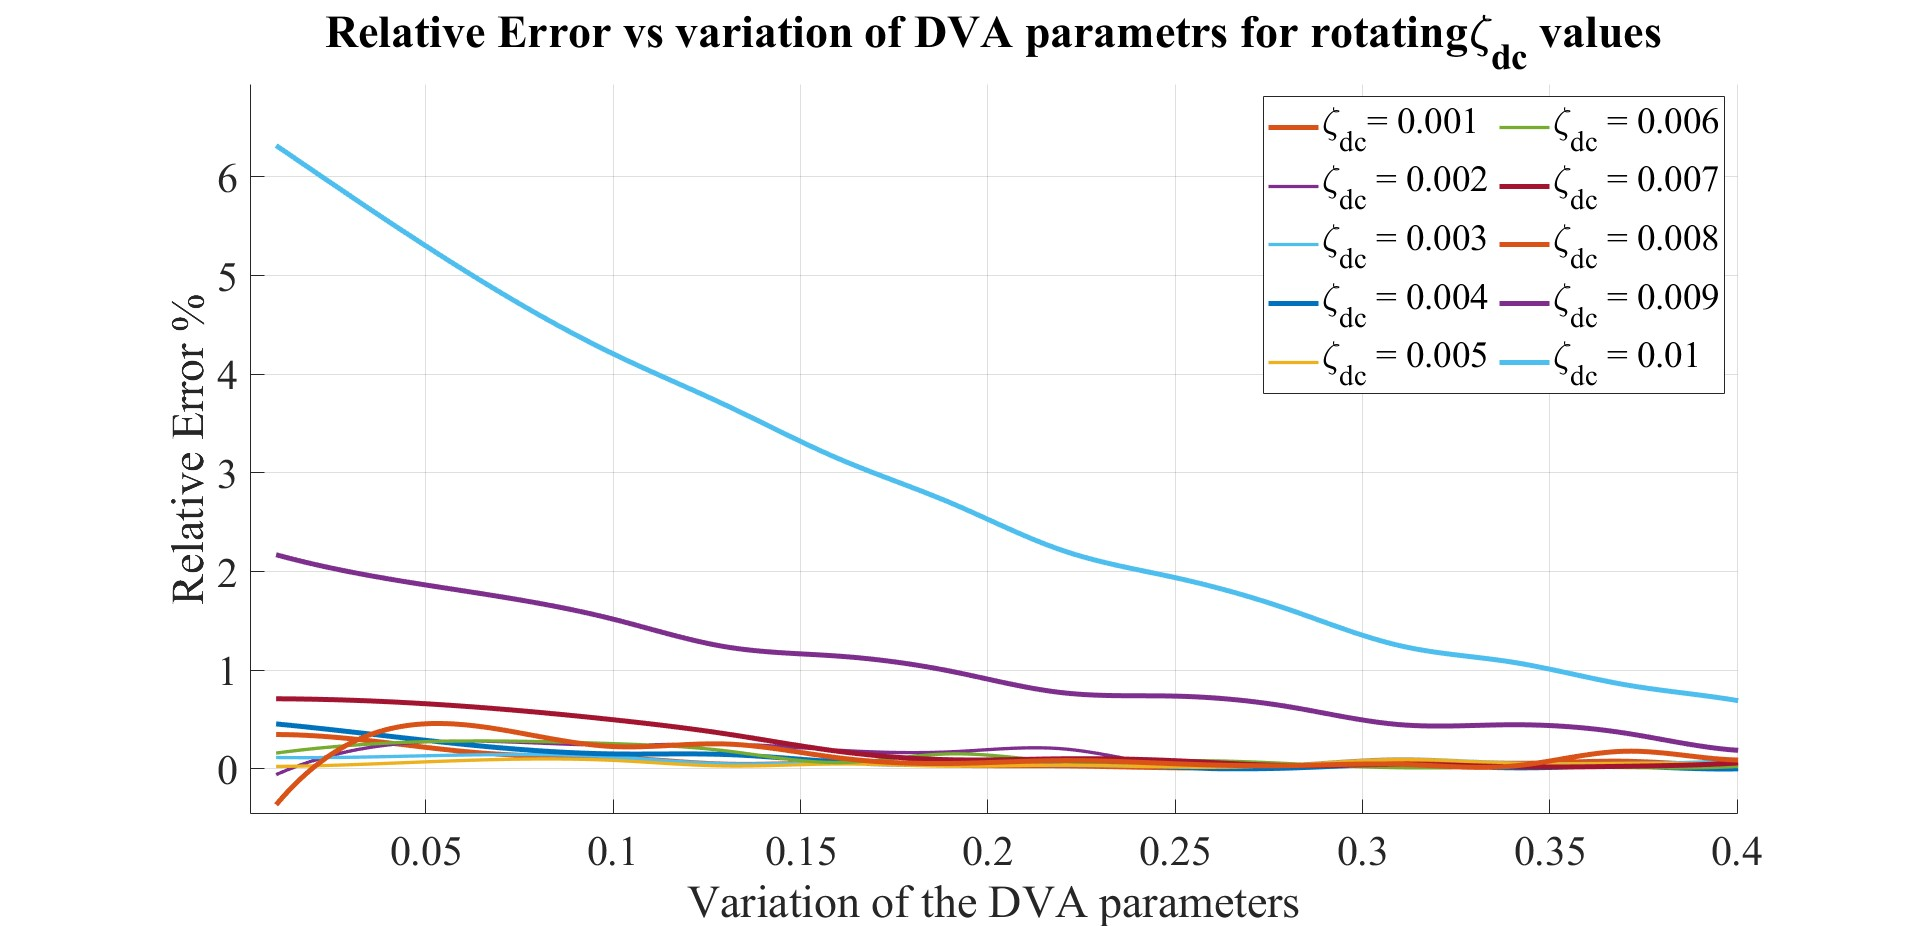
\includegraphics[width=\linewidth]{Fig.sens.zetadc.a.jpg}
    \caption{(الف) بازه $\zeta_{dc}\in[0,\,0.4]$.}
    \label{subfig:zeta_dc_a}
  \end{subfigure}\vfill
  \begin{subfigure}[t]{\linewidth}
    \centering
    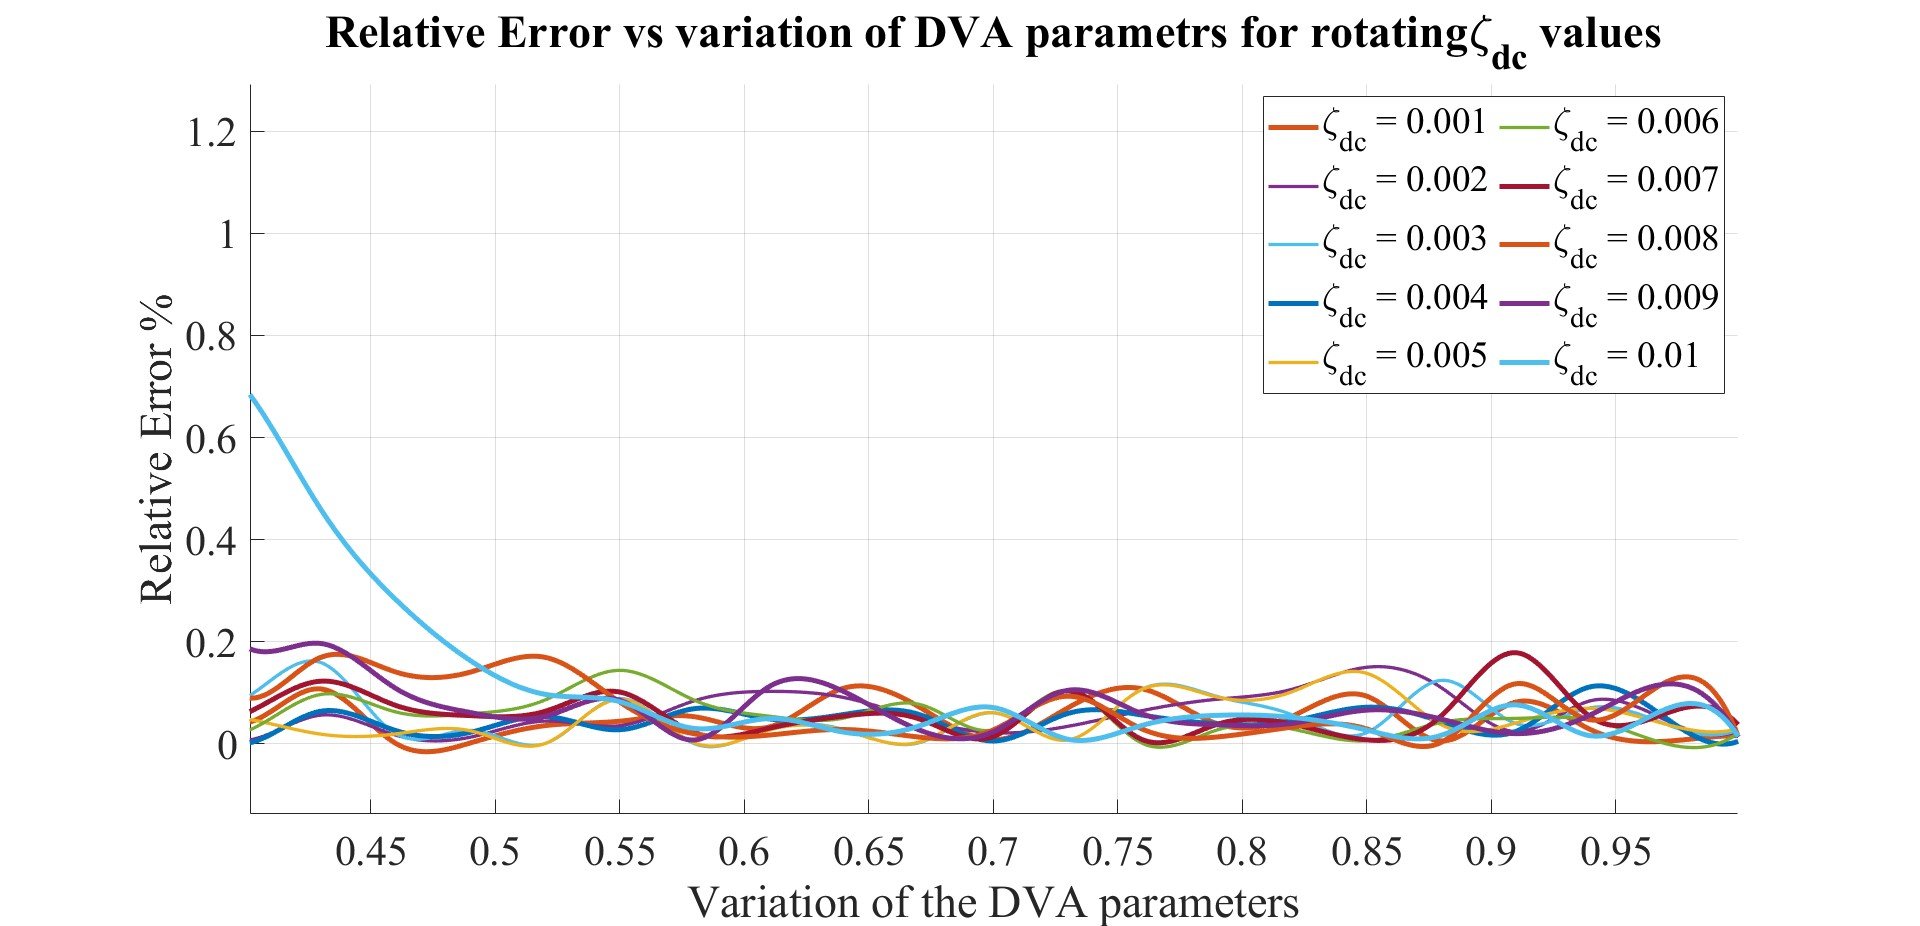
\includegraphics[width=\linewidth]{Fig.sens.zetadc.b.jpg}
    \caption{(ب) بازه $\zeta_{dc}\in[0.4,\,1]$.}
    \label{subfig:zeta_dc_b}
  \end{subfigure}
  \caption{تحلیل حساسیت $\zeta_{dc}$ برای تغییرات مختلف پارامترهای \lr{DVA} در دو بازه متمایز.}
  \label{fig:zeta_ranges}
\end{figure}
% --- پایان بخش ---
